% UCL Thesis LaTeX Template
%  (c) Nicole Mantl, 2022

\documentclass[12pt, english]{report}
\usepackage[utf8]{inputenc}
\usepackage[a4paper, lmargin=4cm, rmargin=2cm, tmargin=1in, bmargin=1in]{geometry}
\usepackage{graphicx}
\usepackage{mathptmx}
\usepackage{amsmath}
\usepackage{gensymb}
\usepackage{indentfirst}
\usepackage{appendix}
\usepackage{helvet}
\usepackage{pifont}
\usepackage{wrapfig}
\usepackage{dirtytalk}
\usepackage{longtable}
\usepackage{fontenc, anyfontsize}
\usepackage{ragged2e}
\usepackage{titletoc}
\usepackage{tocloft}
\graphicspath{ {./graphics/} }

\linespread{1.40}
\setlength{\parindent}{.5cm}

\usepackage{caption}
\captionsetup{font=footnotesize}

\usepackage{subcaption}
\usepackage{array,booktabs,multirow}
\newcolumntype{L}{>{\centering\arraybackslash}m{2.1cm}}
\usepackage{pdflscape}

\usepackage{titlesec}
\titleformat{\chapter}[display]{\normalfont\huge\centering}   {\textbf{\textasteriskcentered{}\ \chaptertitlename\ \thechapter\ \textasteriskcentered{}}}{15pt}{\fontsize{22pt}{20pt}\selectfont}
\titlespacing{\chapter}{0pt}{-32pt}{2cm}
\titleformat{\section}{\scshape\LARGE}{\thesection}{0.3em}{}
\titlespacing{\section}{0pt}{32pt}{.5cm}
\titleformat{\subsection}{\normalfont\Large}{\themysubsection}{0.5em}{}
\titlespacing{\subsection}{0pt}{32pt}{.4cm}
\titleformat{\subsubsection}{\fontsize{16pt}{14pt}\selectfont}{\themysubsubsection}{0.5em}{}
\titlespacing{\subsubsection}{0pt}{32pt}{.3cm}
\titleformat{\paragraph}[hang]{\fontsize{14.5pt}{12pt}\selectfont}{\theparagraph}{0.5em}{}
\titlespacing{\paragraph}{0pt}{32pt}{.2cm}
\titleformat{\subparagraph}[drop]{\itshape\fontsize{13pt}{12pt}\selectfont}{\thesubparagraph}{0.5em}{}
\titlespacing*{\subparagraph}{3cm}{20pt}{.3cm}


\setcounter{secnumdepth}{5}

\usepackage[sorting=none]{biblatex}
\addbibresource{references.bib}




\usepackage{tikz,pgfplots}
\usepackage{pgfplotstable}
\pgfplotsset{compat=1.15}
\usetikzlibrary{shapes.geometric, arrows}
\tikzstyle{startstop} = [rectangle, rounded corners, minimum width=3cm, minimum height=1cm, text centered, draw=black]
\tikzstyle{io} = [trapezium, trapezium left angle=70, trapezium right angle=110, minimum width=4cm, minimum height=1cm, text centered, text width=3.5cm,  trapezium stretches=true, draw=black]
\tikzstyle{process} = [rectangle, minimum width=4cm, minimum height=1cm, text centered, text width=4cm, draw=black]
\tikzstyle{decision} = [diamond, aspect=3, minimum width=3cm, text centered, text width=3.0cm, draw=black]
\tikzstyle{arrow} = [thick, ->, >=stealth]
\usetikzlibrary{positioning, arrows}

\usepackage{abstract}
\renewcommand{\abstractnamefont}{}
\usepackage{etoolbox}
\patchcmd{\abstract}{\null\vfill}{}{}{}

\setcounter{tocdepth}{5}

\renewcommand{\cftchapfont}{\bfseries}
\renewcommand{\cftchappagefont}{\bfseries}
\renewcommand{\cftchappresnum}{Chapter }
\renewcommand{\cftchapnumwidth}{6em}
\renewcommand{\cftsecnumwidth}{1.5em}
\renewcommand{\cftsubsecnumwidth}{2.2em}
\renewcommand{\cftsubsubsecnumwidth}{2.9em}
\renewcommand{\cftparanumwidth}{1.5em}
\renewcommand{\cftsubparanumwidth}{1.5em}
\renewcommand{\cftsubsecindent}{3em}
\renewcommand{\cftsubsubsecindent}{5.2em}
\renewcommand{\cftparaindent}{8.1em}
\renewcommand{\cftsubparaindent}{9.7em}
\renewcommand{\cftfignumwidth}{3em}
\renewcommand{\cfttabnumwidth}{3em}

\cftsetpnumwidth{0cm}
\cftsetrmarg{0.4cm}

\makeatletter
\newcommand*\updatechaptername{%
	\addtocontents{toc}{\protect\renewcommand*\protect\cftchappresnum{\@chapapp\ }}
}
\makeatother

\cftpagenumbersoff{chapter} 
\usepackage{epigraph}

\usepackage{chngcntr}
\counterwithout{equation}{chapter}
\renewcommand{\thechapter}{\Roman{chapter}}
\renewcommand{\thesection}{\arabic{section})}
\renewcommand{\thesubsection}{\themysubsection}
\renewcommand{\thesubsubsection}{\themysubsubsection}
\renewcommand{\theparagraph}{\alph{paragraph}.}
\renewcommand{\thesubparagraph}{--}
\renewcommand{\thefigure}{\Roman{chapter}.\arabic{figure}}
\renewcommand{\thetable}{\Roman{chapter}.\arabic{table}}

\newcommand{\themysubsection}{\arabic{section}.\arabic{subsection}}
\newcommand{\themysubsubsection}{\arabic{section}.\arabic{subsection}.\arabic{subsubsection}}

\usepackage{url}

%% Define a new 'leo' style for the package that will use a smaller font.
\makeatletter
\def\url@leostyle{%
  \@ifundefined{selectfont}{\def\UrlFont{\sf}}{\def\UrlFont{\footnotesize\sffamily}}}
\makeatother
%% Now actually use the newly defined style.
\urlstyle{leo}

\newcommand\mysection[2]{\section[#1]{#1\hrulefill}}

\newcommand\Section[2]{\section[#1: {#2}]{#1\hrulefill\\[-2ex]\normalsize\itshape#2}}

\newcommand\Chapter[2]{\chapter[\textsl{#1: {#2}}]{\textsl{#1}\\[1ex]\Large{#2}}}

\begin{document}
%TC:ignore
\begin{titlepage}

   \begin{center}
       \vspace*{3cm}
       {Simulating Gravity Assists in Python}
 
       \vspace{4cm}
 
       {21018444}\\
       
       \vspace*{10cm}
      
       
      UCL\\
      
      BSc Theoretical Physics\\
      
      2023
      
 
   \end{center}
\end{titlepage}

\setcounter{page}{2}
\noindent 
\chapter*{\huge{\textbf{Abstract}}}
\normalsize{\noindent A gravity assist, or gravitational slingshot, is a complex maneuver which allows for an object to alter its velocity by entering another object's gravitational field. This project uses classical mechanics and the velocity Verlet algorithm to model a gravity assist in numerous scenarios, beginning with the modelling of a three-body system and the testing of the Runge-Kutta integrator, with the aims of understanding how this complex maneuver can be simulated in a high-level programming language. Some limitations became apparent early into the investigation, mainly involving computational power, but the project culminated in a four-body system where a satellite underwent a series of gravity assists from Jupiter and Saturn. It was found that the simulation of an object undergoing gravity assists in Python is highly feasible.}
%\input{}


%\input{}


\setlength{\cftbeforetoctitleskip}{-22pt}
\setlength{\cftaftertoctitleskip}{-22pt}
\renewcommand{\contentsname}{\huge\textbf{Table of Contents}}
\renewcommand{\cfttoctitlefont}{\chapter*}

\tableofcontents

\clearpage

\setlength{\cftbeforeloftitleskip}{-22pt}
\renewcommand{\cftloftitlefont}{\hfill\huge\bfseries}
\renewcommand{\cftafterloftitle}{\hfill}
\listoffigures

\clearpage

%\setlength{\cftbeforelottitleskip}{-22pt}
%\renewcommand{\cftlottitlefont}{\hfill\huge\bfseries}
%\renewcommand{\cftafterlottitle}{\hfill}
%\listoftables


%TC:endignore
\cleardoublepage

\chapter{\textsl{Introduction}}
\normalsize{\noindent For an object with no forces acting on it, some form of propellant, or some work done, is required such that its velocity is altered. This comes as a result of Newton's First Law \cite{newton_principia_1999}, which states that any object any object at rest or in uniform motion will continue to do so unless a force is applied to it. Considering now a satellite with a finite amount of propellant, planning its route through space becomes an exigent task that requires the perfect management of fuel and necessitates even larger fuel payloads, both of which add extra costs and labour to the already expensive missions.

Thankfully, prior to the launch of the first man-made satellite even, scientists were already thinking about how to navigate the cosmos in a fuel-free way. The earliest descriptions of this came from Yuri Kondratyuk \cite{noauthor_kondratuk_nodate}, a Russian scientist whose early works explored the idea of using a planet's moons to accelerate an object. After many more expanded upon this idea, the first attempt of a "gravity assist" was carried out by the Soviet Union with the Luna 3 probe successfully photographing the far side of the Moon \cite{noauthor_luna_nodate}. Later, NASA's Pioneer 10 successfully used the technique to increase velocity from 52,000 km/h to 132,000 km/h \cite{administrator_pioneer_2015}.}



%\input{}

%\chapter{\textsl{Literature/Systematic Review}}
\chapter{\textsl{Methods}}

\section{\textsl{Preliminary investigation: n-body orbits}}
\subsection{\textsl{Three-body velocity Verlet}}

\normalsize{\noindent First, it was necessary to model a three-body system using Matplotlib. This began by considering Newton's Law of Gravitation \cite{newton_principia_1999}

\begin{equation} \label{eq:1}
    \vec{F} = \frac{GMm}{r^2} \hat{r},
\end{equation}
to determine the gravitational force between two objects with masses $M$ and $m$ and separated by distance $r$.} By equating this to the equation for centripetal force \cite{newton_principia_1999} \begin{equation}
    \vec{F} = \frac{mv^2}{r} \hat{r}
\end{equation}

where $v$ corresponds to the tangential velocity and rearranging, one obtains 
\begin{equation} \label{eq:3}
    v = \sqrt{\frac{GM}{r}},
\end{equation}

which describes the velocity required for a circular orbit around an object of mass $M$ at distance $r$, or otherwise known as the \emph{orbital velocity}. Equation \ref{eq:3} was used extensively throughout when concerning an arbitrary initial position and assigning an initial velocity to a planet in a circular orbit. 

% insert something here about orbital mechanics, specifically about velocity increase or something idk

\normalsize{When it came to propagating the orbits through time, two approaches were carried out. Initially the velocity Verlet integrator \cite{bowler_phas0030_nodate} was used. Given a position $x(t)$ and velocity $v(t)$, the propagation of these quantities by a quantity $\Delta t$ can be expressed as 
\begin{align}
    x(t + \Delta t) &= x(t) + v(t)\Delta t  + \frac{F(t)}{2m} \Delta t^2 \\ 
    v(t + \Delta t) &= v(t) + \frac{F(t) + F(t + \Delta t)}{2m} \Delta t,
\end{align} where $F(t)$ and $m$ is the force on and mass of the object being simulated.}

\normalsize{Using Equation \ref{eq:3}, and some simulation parameters closely resembling the Sun, Earth, and Moon, the initial velocity was calculated of the Earth by considering the velocity of the Sun only. The velocity of the Moon relative to the Earth was also calculated using Equation \ref{eq:3}, ignoring the effects of the Sun. Then, the initial velocity of the Earth was added to this to determine the initial velocity of the Moon.

To check that the law of conservation of energy \cite{noauthor_feynman_nodate} was obeyed throughout each simulation, the kinetic energy \cite{noauthor_210_2018}

\begin{equation}
    K = \frac{1}{2} \sum^n_i m_i v_i^2,
\end{equation}
}
was calculated for each planet and summed (the Sun was kept stationary throughout each simulation so it was not accounted for). 

\subsection{\textsl{Two-body Runge-Kutta}}
\normalsize{\noindent In the search for a better integrator, the fourth-order Runge Kutta integrator was used. This required the decomposition of the equation of motion to form two coupled first-order equations from a second-order equation. Starting from Equation \ref{eq:1}, one can divide both sides by $m$ and rearrange as follows
\begin{align}
    a &= \frac{GM}{r^2} \\
    \frac{d^2x}{dt^2} &= \frac{GM}{r^2}.
\end{align}
Hence, two coupled first order differential equations are obtained:
\begin{align}
    \frac{dx}{dt} &= v \\
    \frac{dv}{dt} &= \frac{GM}{r^2}.
\end{align}
Both of these equations were then passed into the RK solver, which enabled the propagation of the simulation. The algorithm of the integrator \cite{bowler_phas0030_nodate}
\begin{align}
\begin{matrix} 
y(x+\mathrm{\Delta x})&=&y(x)+\frac{1}{6}\left(k_1+2k_2+2k_3+k_4\right)\\k_1&=&\mathrm{\Delta x}\ f(x,y(x))\\k_2&=&\mathrm{\Delta x}\ f(x+\mathrm{\Delta x}/2,y(x)+k_1/2)\\k_3&=&\mathrm{\Delta x}\ f(x+\mathrm{\Delta x}/2,y(x)+k_2/2)\\k_4&=&\mathrm{\Delta x}\ f(x+\mathrm{\Delta x},y(x)+k_3) \end{matrix}
\end{align}

was written in Python, and a two-body system was modelled using this. Given some setbacks with the usage of the RK4 solver to model a three-body system and the perceived adequacy compared to its simplicity of the Verlet integrator, the project continued with the latter.}

\section{\textsl{Further investigation: gravity assists}}
\subsection{\textsl{Simple gravity assist using Earth}}

\normalsize{\noindent A \emph{gravity assist} is a maneuver that results in a change in velocity of an object when it enters the sphere of influence of another object \cite{noauthor_basics_nodate}. The \emph{radius of the sphere of influence} $r_{\mathrm{SOI}}$  \cite{noauthor_sphere_nodate} is calculated by
\begin{equation}
    r_{\mathrm{SOI}} \approx a\left( \frac{m}{M} \right)^{2/5}.
\end{equation}

\noindent Using the same masses as previously, but this time changing the Moon's mass to be closer to that of a satellite (approximated to be 1 tonne), the values for $r_{\mathrm{SOI}}$ were calculated for both the Sun and Earth. This was taken into consideration when choosing the path for the satellite to take, since selecting a path that placed it outside of the Earth's SOI would result in no velocity change at all. 

To begin with, the influence of the Sun on the satellite's motion was neglected, and the satellite was given an arbitrary position outside of the Earth's sphere of influence. In order to allow the satellite to intersect the Earth's orbit at an arbitrary point, the simulation was ran to determine the time taken $t$ for Earth to reach said point. Then, using the fact that for constant acceleration $v = \Delta r / \Delta t$ \cite{newton_principia_1999} the initial velocity of the satellite was calculated to be 
\begin{equation}
    \vec{v_0} = \frac{(r_{\mathrm{IP}} - r_0)}{t},
\end{equation}
\indent where $r_{\mathrm{IP}}$ and $r_0$ are the positions of the satellite near the interception point and at the start of the simulation. The interception point was perturbed by a small amount (still ensuring that it was not outside the sphere of influence of Earth), such that in one case it passed in front of the Earth, and in another case behind it. This is due to the idea that passing in front or behind an object can have different effects for the final velocity of the object. To be specific, passing behind the object, results in an increase in velocity, and the opposite occurs for passing in front of it. It is worth noting that the object's velocity remains the same in the assisting body's (in this case Earth's) frame of reference, but will be altered in other (in this case the Sun's) frame(s) of reference. In order to understand this, a quick overview of hyperbolic orbits is required.
\begin{figure}[ht]
    \centering
    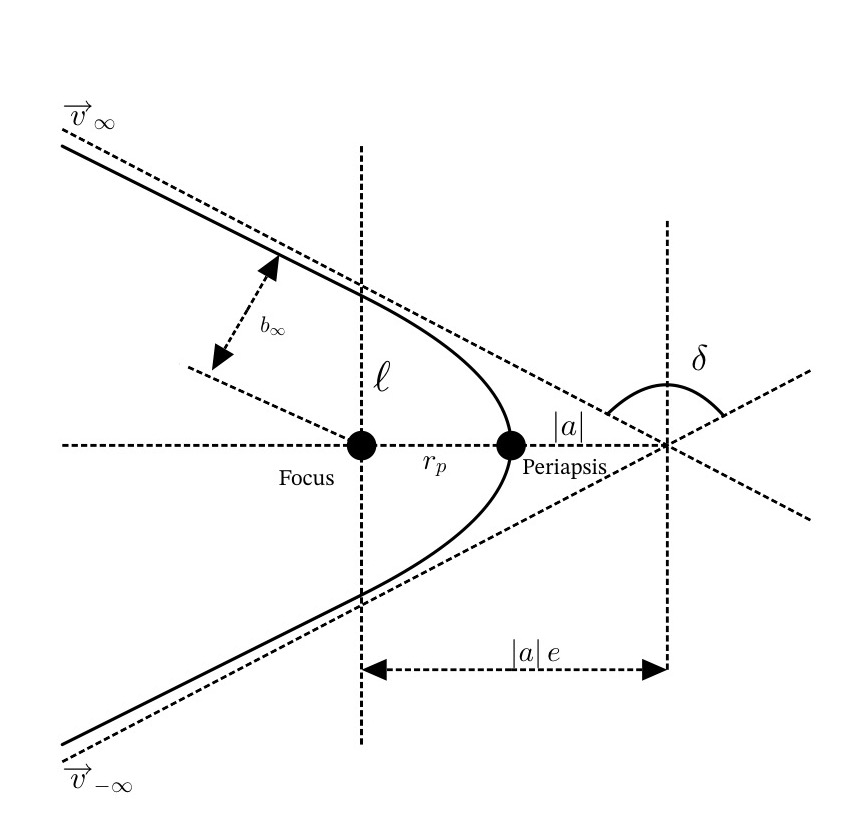
\includegraphics[width=0.6\textwidth]{graphics/Orbits.jpg}
    \caption{Diagram showcasing a hyperbolic orbit}
    \label{fig:hyp_orbit}
\end{figure}

Quite simply, a hyperbolic orbit around an object resembles a hyperbole in the object's frame of reference and has an eccentricity $e > 1$ \cite{kluever_spaceflight_2003}. For the object in the hyperbolic orbit, two asymptotes can be constructed which intersect at point $O$, distance $a$ from the periapsis of the orbit, and a line drawn parallel to the asymptote from the centre of the orbit is distance $b$ from the asymptote . This is illustrated in Figure \ref{fig:hyp_orbit} . At an infinite distance along each asymptote, the \emph{Entering and Exiting Hyperbolic Excess Velocity} $\vec{v_{\mp \infty}}$ is defined , with the difference between the two
\begin{equation} 
    \vec{v_{\infty}} - \vec{v_{-\infty}} = \Delta \vec{v},
\end{equation}
corresponding to the change in velocity in the reference frame of the body that the object is orbiting.
}

In the case of the satellite passing in front of Earth, it encounters a gravitational "headwind" as a result of the force from Earth on the satellite that reduces the exiting hyperbolic excess velocity, resulting in a negative change in velocity. Conversely, the satellite passing behind Earth experiences a gravitational "tailwind" that increases the exiting hyperbolic excess velocity, resulting in a positive change in velocity. It is with this idea that two cases of gravity assists were attempted.

\subsection{\textsl{Swapping Earth for Jupiter}}
\normalsize{\noindent After a gravity assist using Earth was modelled, Earth was swapped for Jupiter to create a larger slingshot. A similar approach was taken to initialising the two-body orbit, with the mass of the second object adjusted this time to be much larger (closer to the mass of Jupiter). Other variables like $r_\mathrm{{SOI}}$ were also calculated so that they could be used for the adjustment of initial velocity.
Following this, the satellite was moved closer to Jupiter (which in conjunction resulted in the reduction of Jupiter's initial velocity) so that the effects at the lower velocity could be gauged.
}

\subsection{\textsl{Including the influence of the Sun}}
\normalsize{\noindent Keeping Jupiter as the planet that will perform the gravity assist, the force from the Sun on the satellite was once again considered. The satellite's position was once again arbitrarily selected, but the initial velocity required recalculation. In order for it to reach the same interception point, either an elliptical, parabolic, or hyperbolic orbit was required.

The \emph{eccentricity} of an orbit \cite{kluever_spaceflight_2003} is defined to be
\begin{equation}
    e = \frac{\ell}{r_p} - 1,
\end{equation}
\indent with $\ell$ and $r_p$ representing the \emph{semi-latus rectum} and \emph{periapsis distance} respectively, both of which are labelled on Figure \ref{fig:hyp_orbit}. Given the selection of the positions of the satellite at time $t=0$ and the interception point, the eccentricity of this orbit $e=1$, which denotes a parabolic orbit. The tangential velocity of this orbit is denoted by 
\begin{equation}
    v = \sqrt{\frac{2\mu}{r}},
\end{equation}
\indent where the \emph{standard gravitational parameter} $\mu$ is approximated to be equal to $GM$. Though assigning this velocity to the satellite allowed it to reach the interception point, it did so much quicker than Jupiter. As such, the deployment and subsequent injection of the satellite had to be delayed to ensure that it and the planet both reached the interception point at the same time. This was done by finding the difference in time taken for Jupiter and the satellite to reach the interception point, and fixing the satellite's position for this duration. This could be thought of as analogous to deploying the satellite with the right timing to intercept Jupiter directly. This time, the lag was perturbed to allow for the satellite to pass behind and in front of the planet.
}

\subsection{\textsl{Double slingshot}}
\normalsize{\noindent After simulating a slingshot from Jupiter, the final part of the further investigation included attempting a slingshot from two planets. The code from the previous part was reused once again, but this time another planet, this time Saturn, was introduced. It was given a mass and orbital radius approximately similar to real life values. After giving it an arbitrary starting position, the second interception point, this time of the satellite and Saturn, was determined. A similar approach was taken to the previous simulation, where this time the planet was held in a stationary position as to allow it and the satellite to reach the interception point at the same time. The lag of Saturn was perturbed accordingly.

}


%\input{}

%\chapter{\textsl{Empirical chapter}}
\chapter{\textsl{Results and Discussion}}
\section{\textsl{Preliminary investigation}}
\begin{figure}[ht]
    \centering
    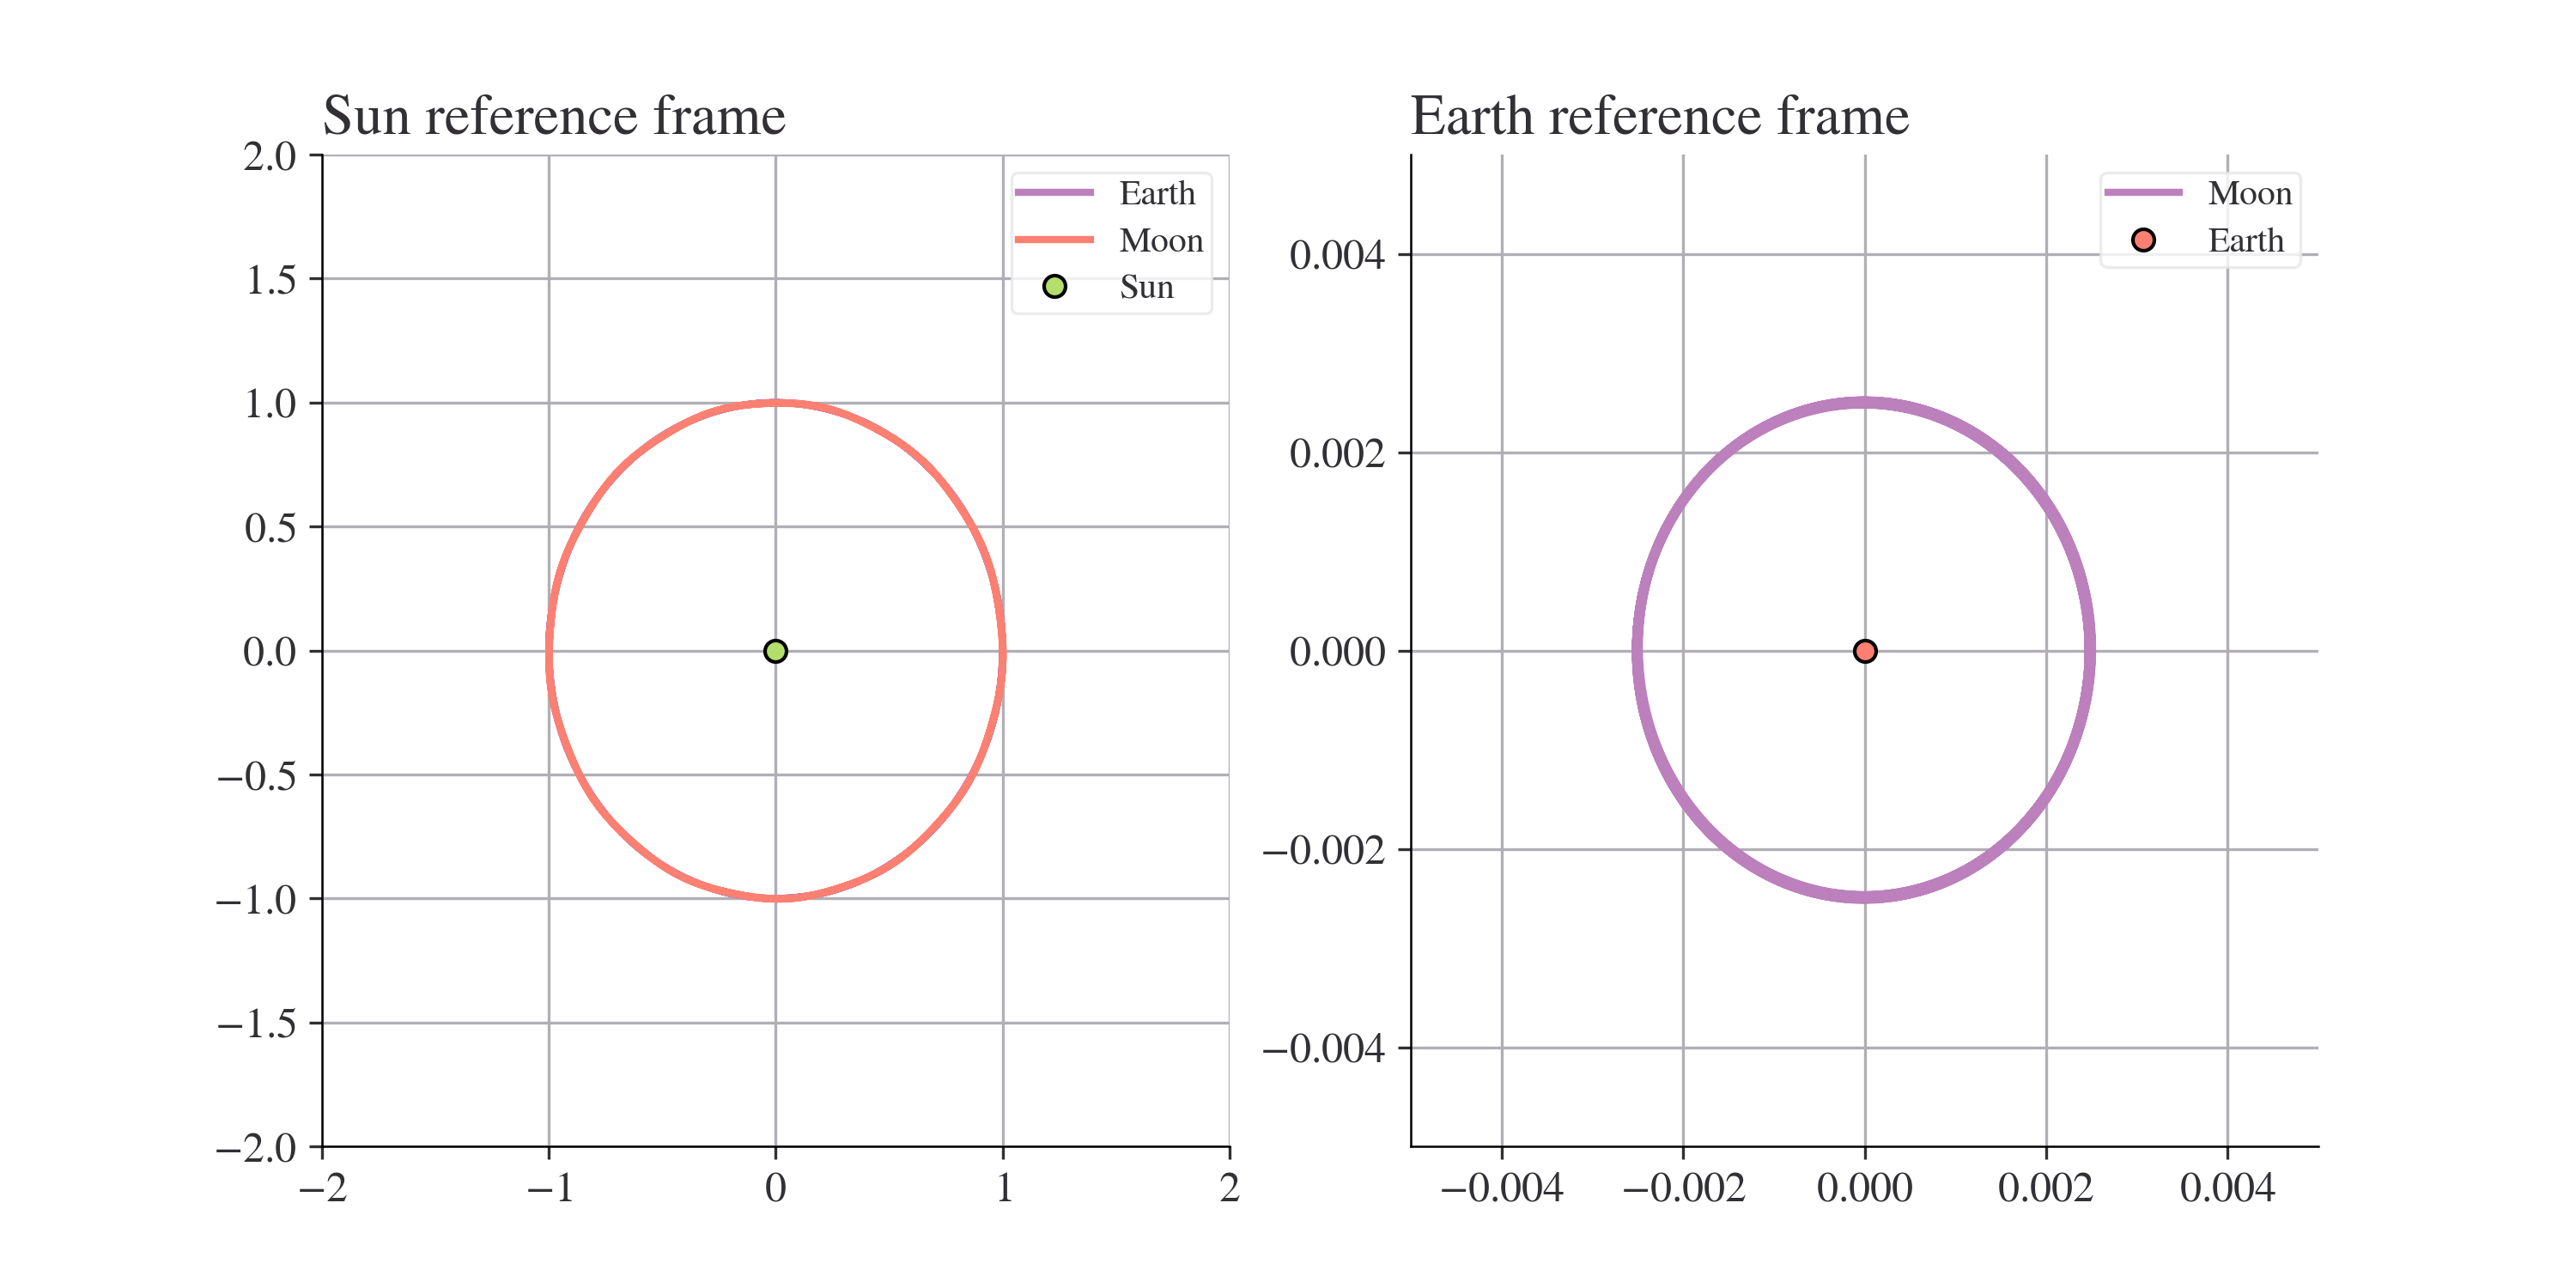
\includegraphics[width=0.7\textwidth]{graphics/3b_verlet.png}
    \caption{3-body velocity Verlet}
    \label{fig:3b_verlet}
\end{figure}

\normalsize{\noindent The velocity Verlet integrator was proven to work sufficiently well when it came to modelling the three-body orbit. As can be seen from Figure \ref{fig:3b_verlet}, both orbits were stable, but there is a noticeable thickness to the orbit of the Moon around the Earth which is an indication of some error in the simulation.
\begin{figure}[ht]
    \centering
    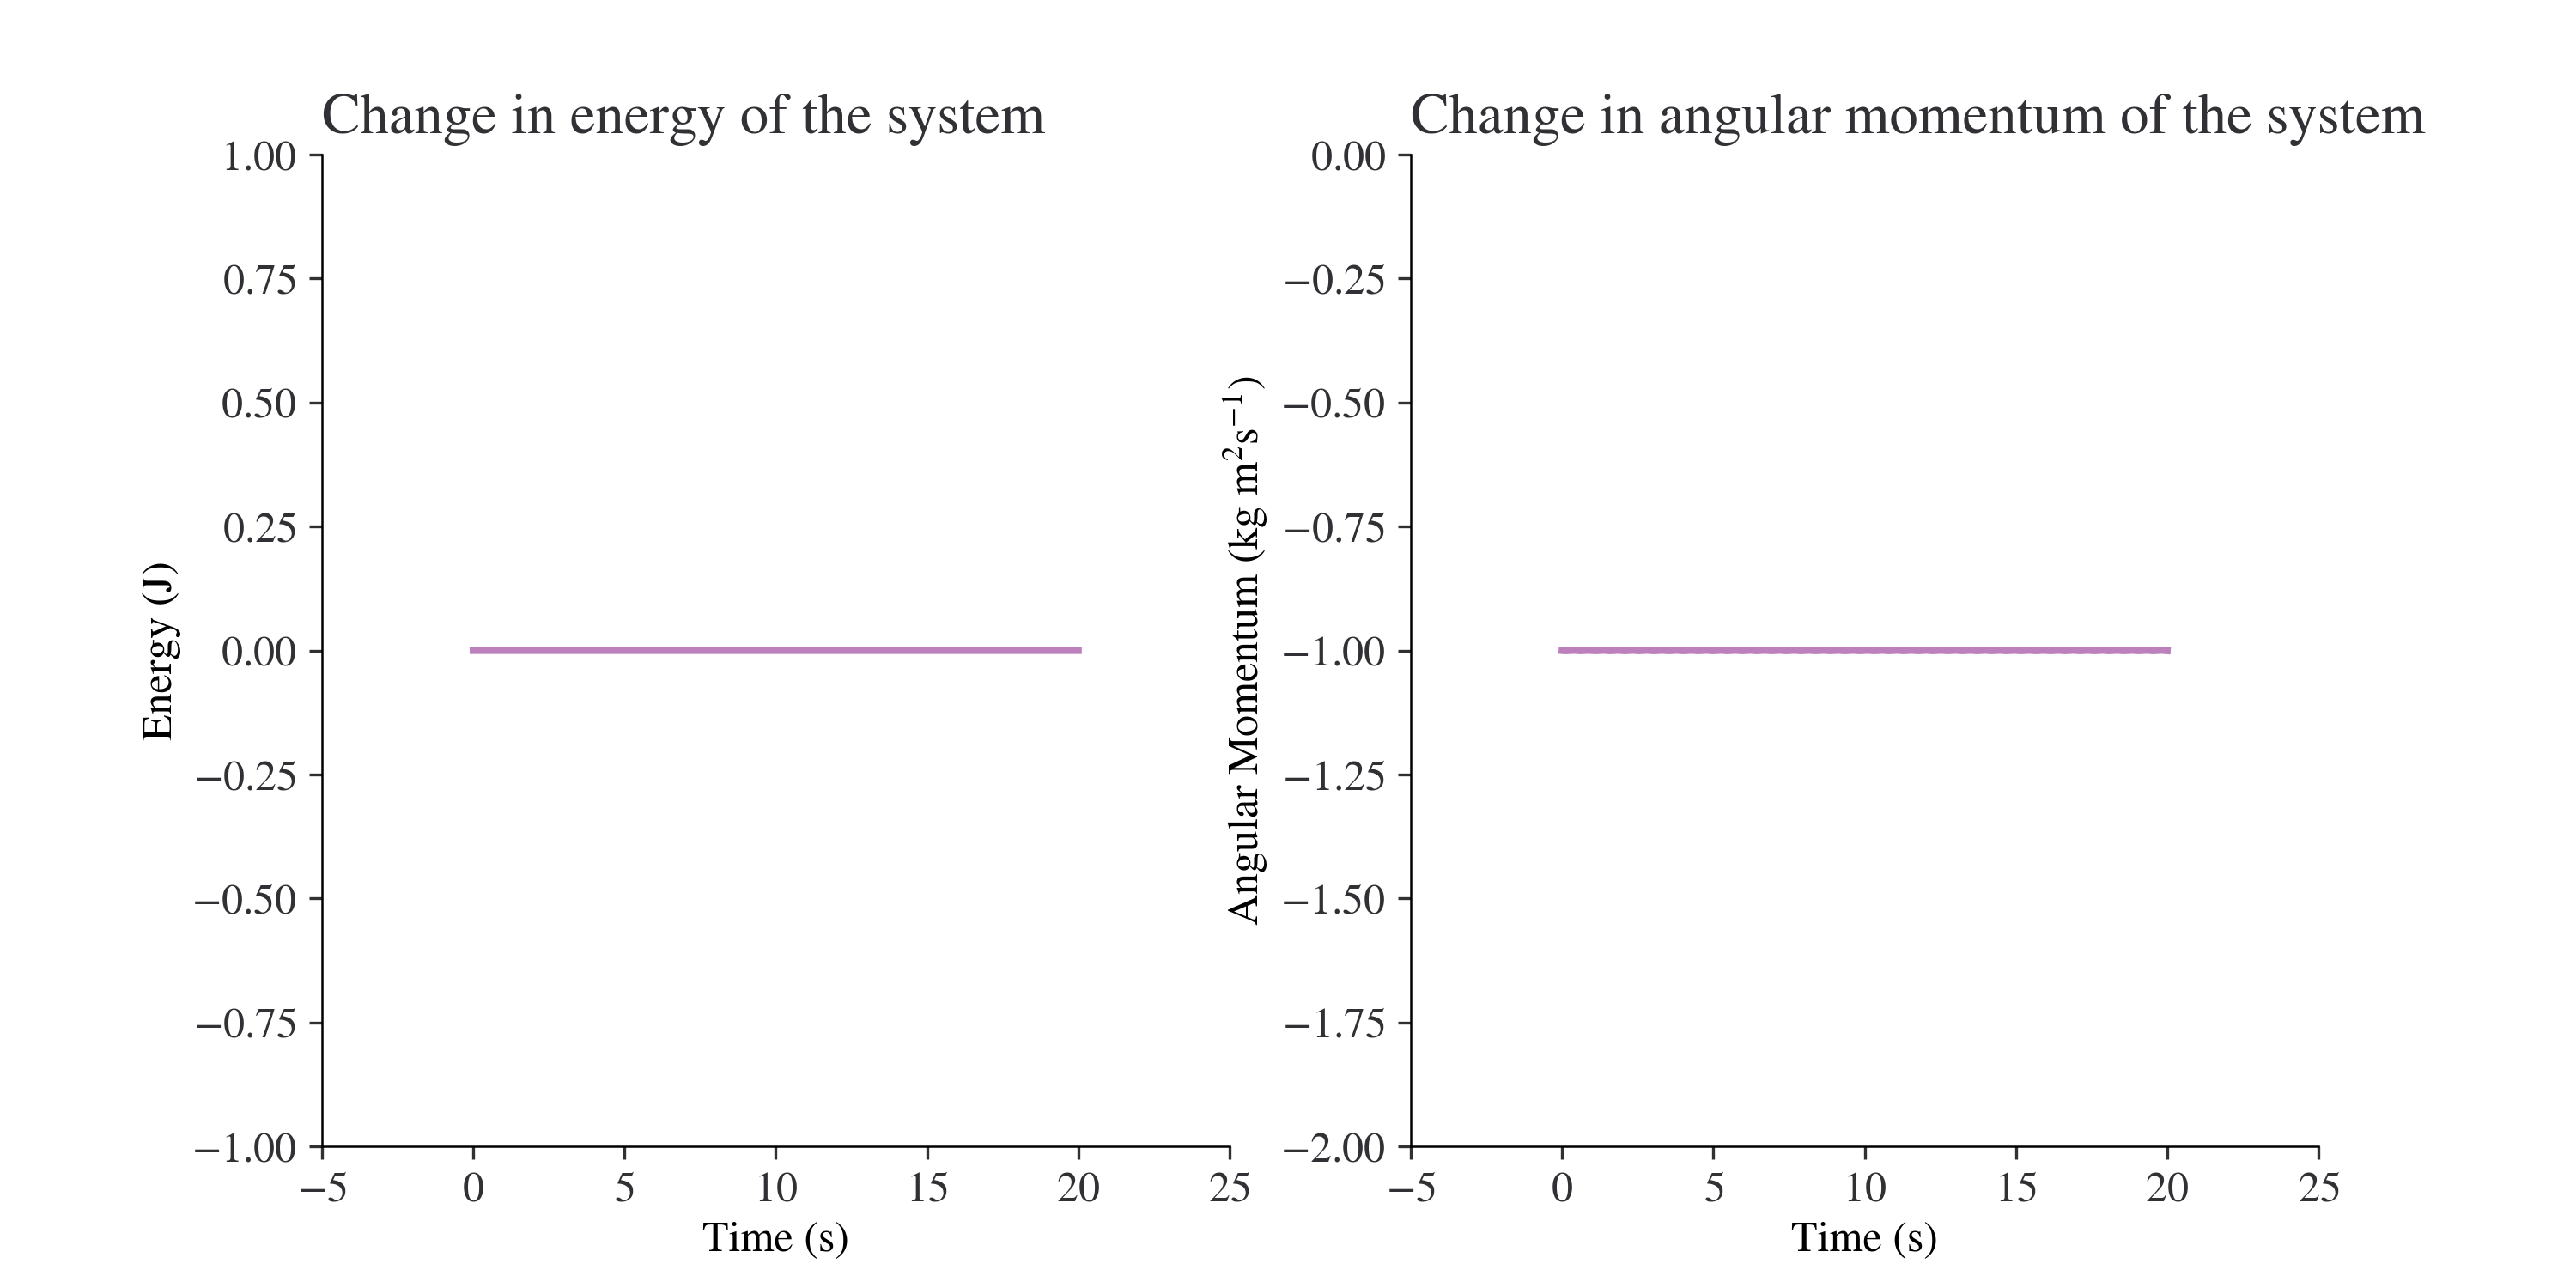
\includegraphics[width=0.6\textwidth]{graphics/3b_conservation.png}
    \caption{Graph depicting the conservation of energy with the Verlet integrator}
    \label{fig:3b_conservation}
\end{figure}

Likely arising from the minor fluctuations in orbital radius that appear in Figure \ref{fig:3b_verlet}, total energy also fluctuates in a sinusoidal manner and on a very small scale. However, as is shown in Figure \ref{fig:3b_conservation}, the total energy does not show an increase over time, therefore demonstrating that this simulation does not violate the law of conservation of energy.}

\normalsize{Moving on to the implementation of the RK4 integrator, it was noticeably more complex than the Verlet integrator. Nonetheless this integrator was used to successfully model a two-body system with the Sun and Earth.}
\begin{figure}[ht]
    \centering
    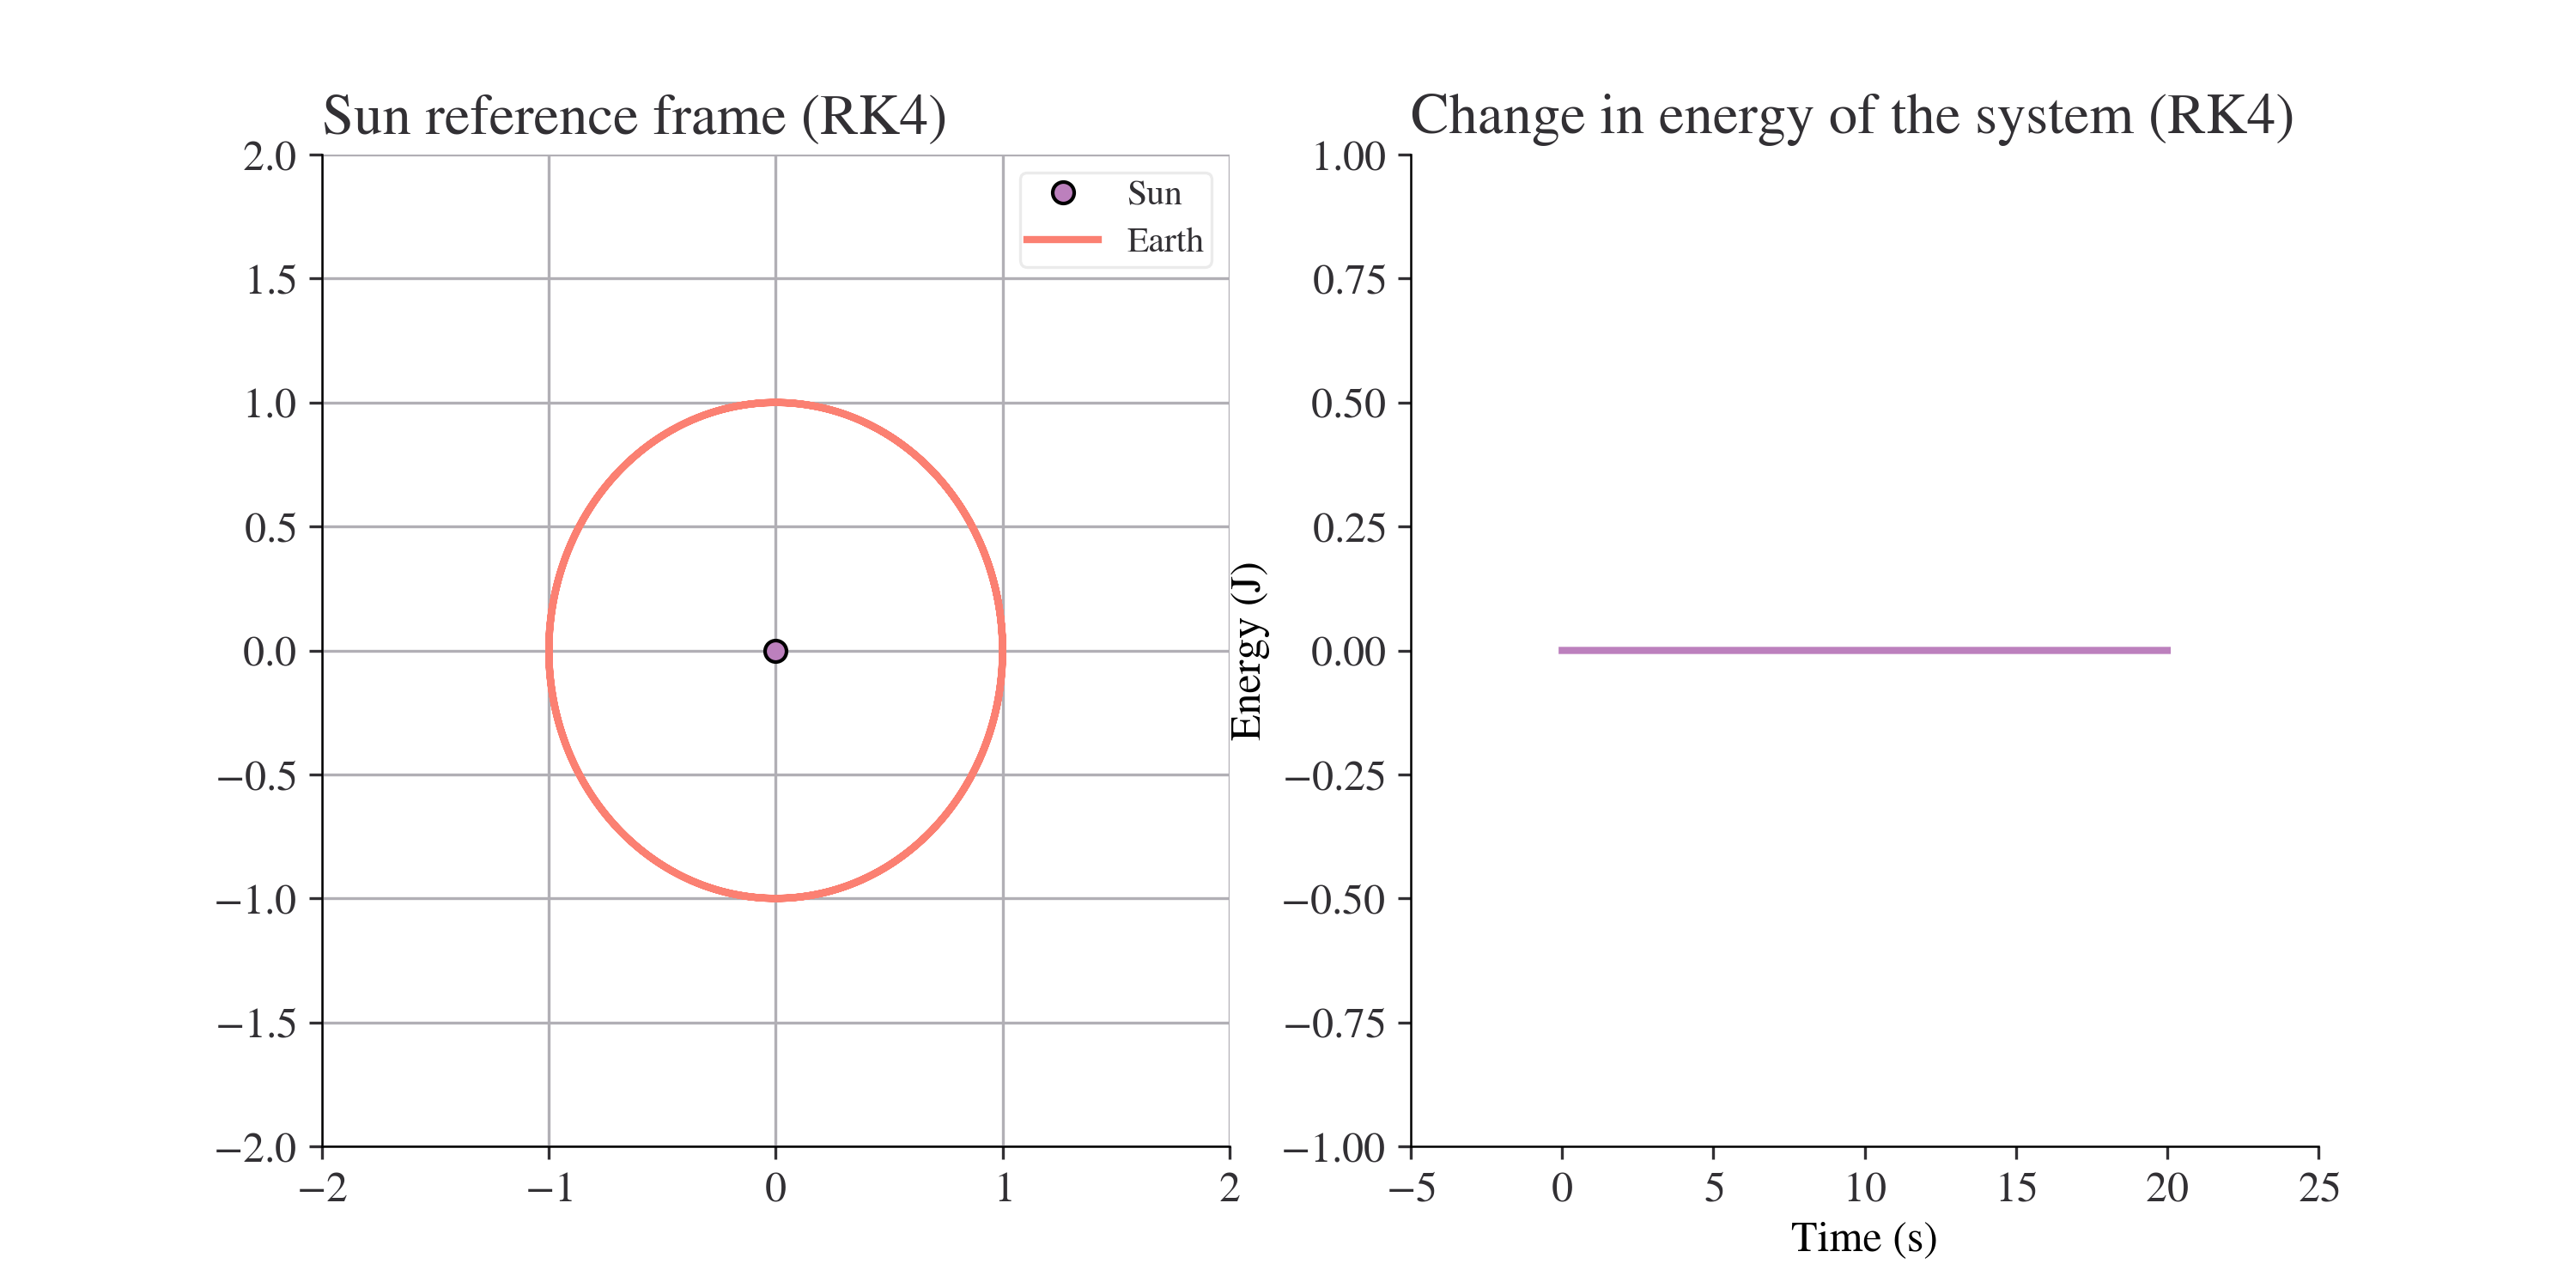
\includegraphics[width=0.8\textwidth]{graphics/rk4.png}
    \caption{2-body Runge-Kutta simulation with conservation of energy}
    \label{fig:rk4}
\end{figure}
\normalsize{
As Figure \ref{fig:rk4} demonstrates, the RK4 solver is a good tool for modelling the two-body problem, as it provides a stable orbit and energy is a conserved quantity. With that said, adding in a third body provided some difficulties that were not encountered during the programming of the velocity Verlet integrator. Mainly, it was difficult to include the interactions between the Moon and the Earth, given that the Earth's orbit had to be calculated beforehand, and a separate solver function had to be defined to resolve this issue. This was not pursued due to time constraints, but a future approach involving the Runge-Kutta integrator could harness the object-oriented programming paradigm to greatly simplify the problem.}

\section{\textsl{Further investigation}}

\begin{figure}[ht]
    \centering
    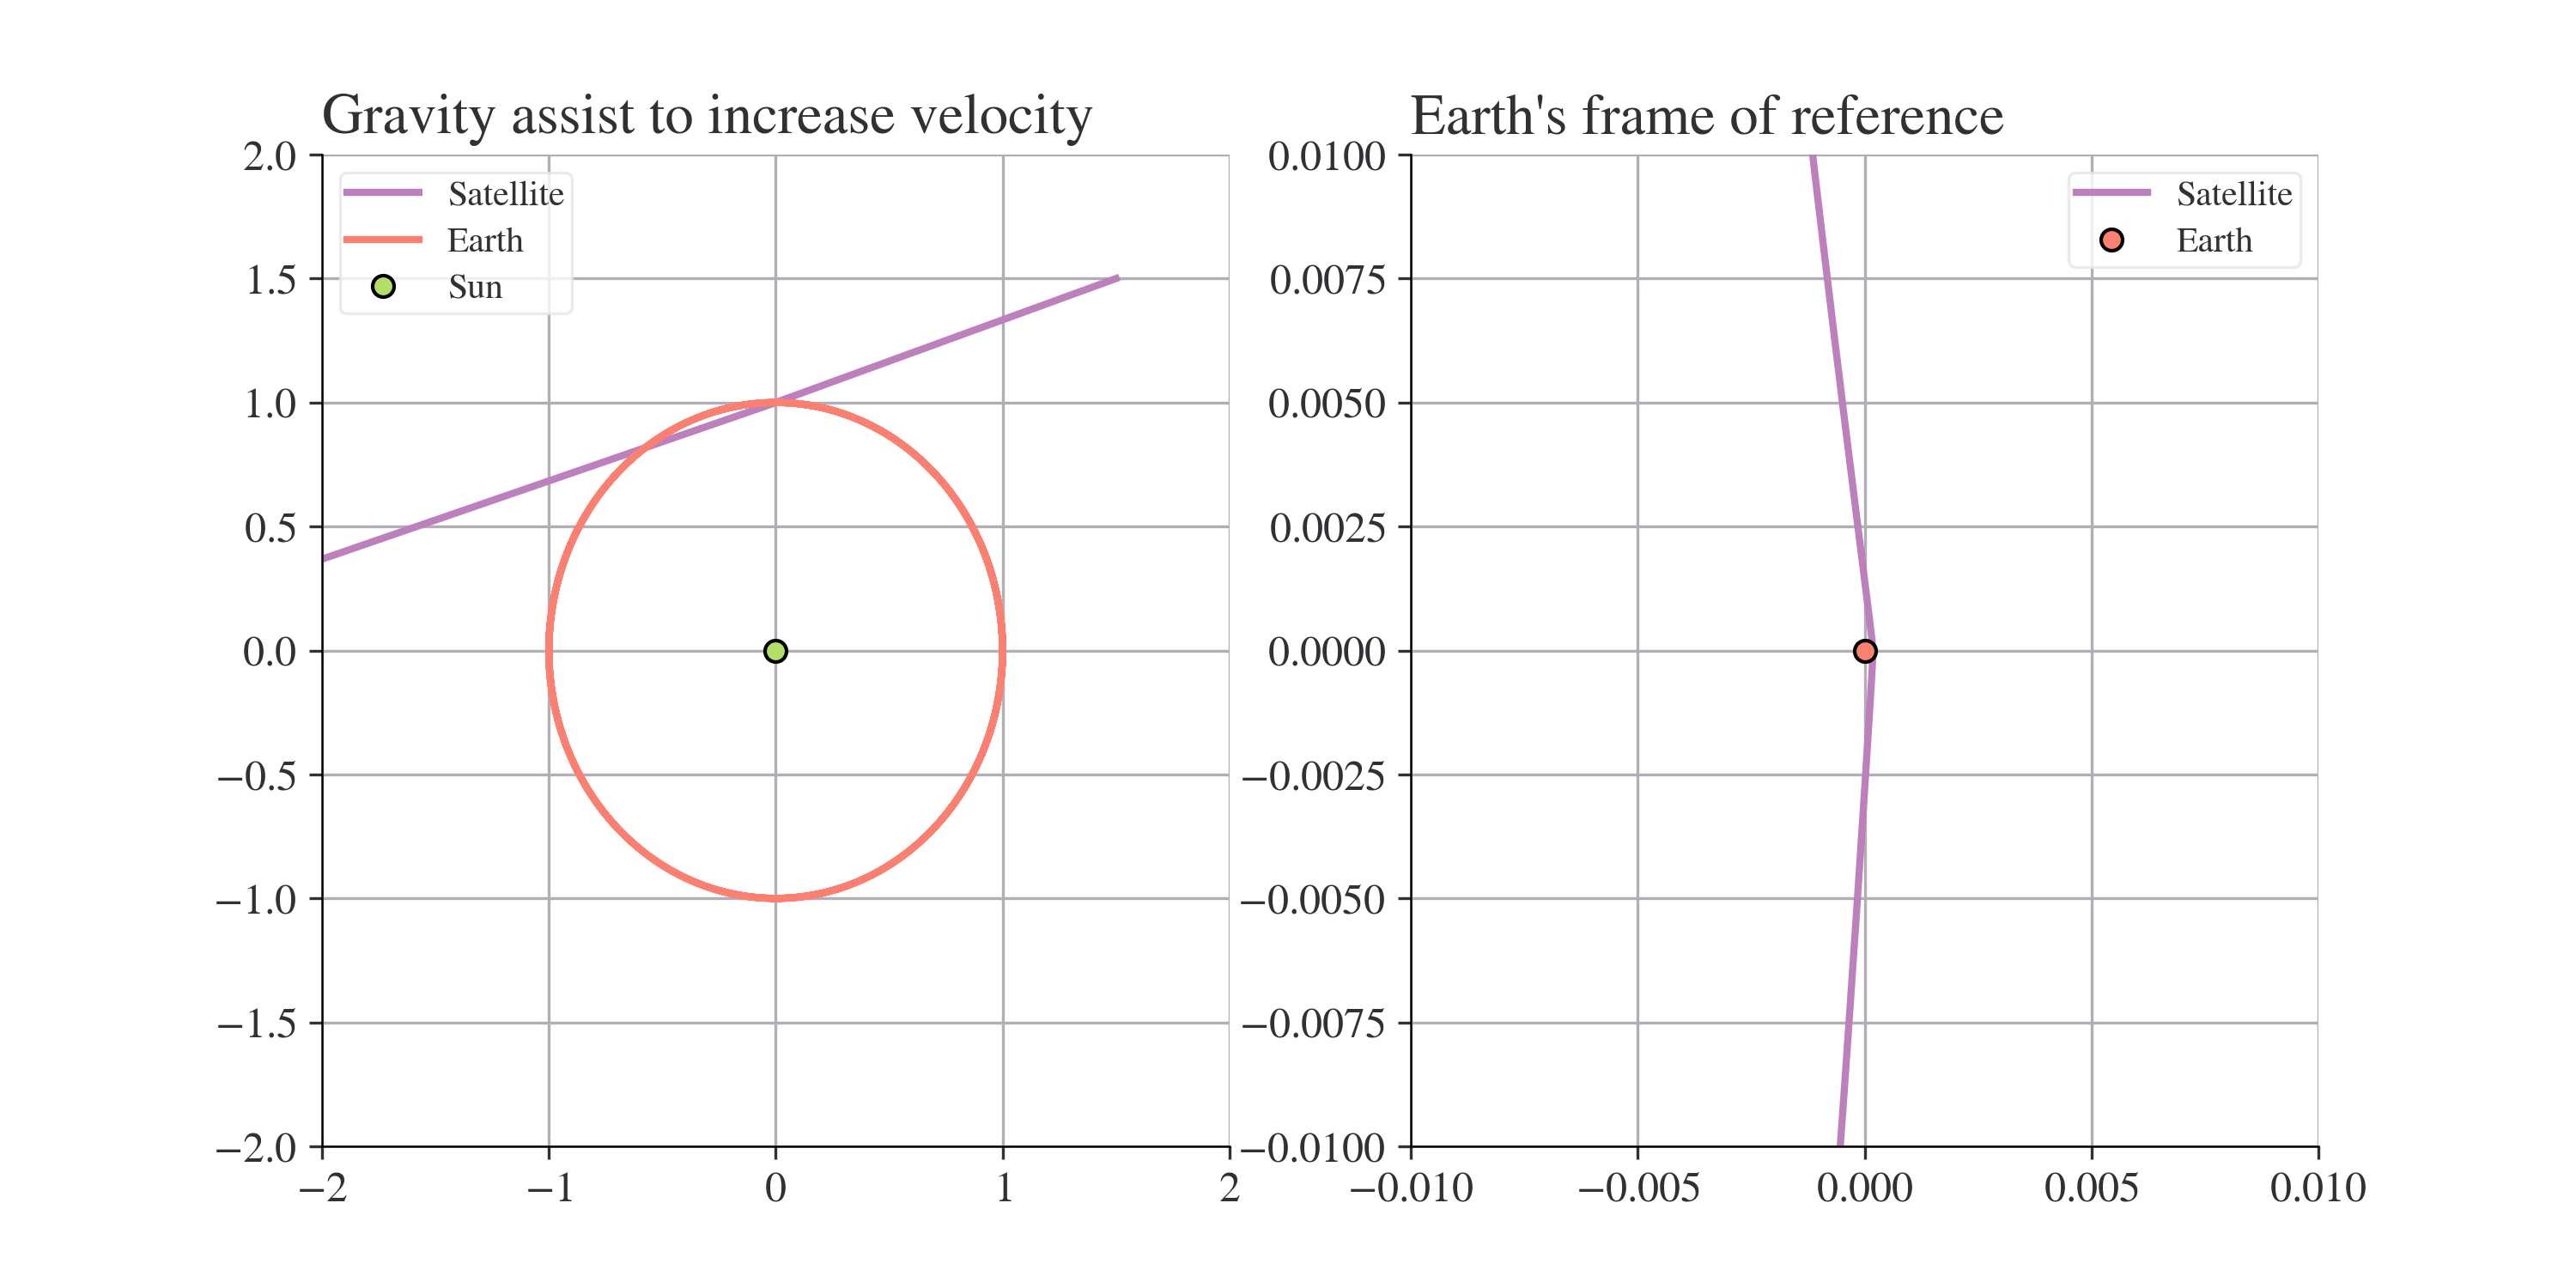
\includegraphics[width=0.7\textwidth]{graphics/earth_increase1.png}
    \caption{Gravity assist between the satellite and Earth resulting in a velocity increase of the satellite}
    \label{fig:earth_increase1.png}
\end{figure}

\begin{figure}[ht]
    \centering
    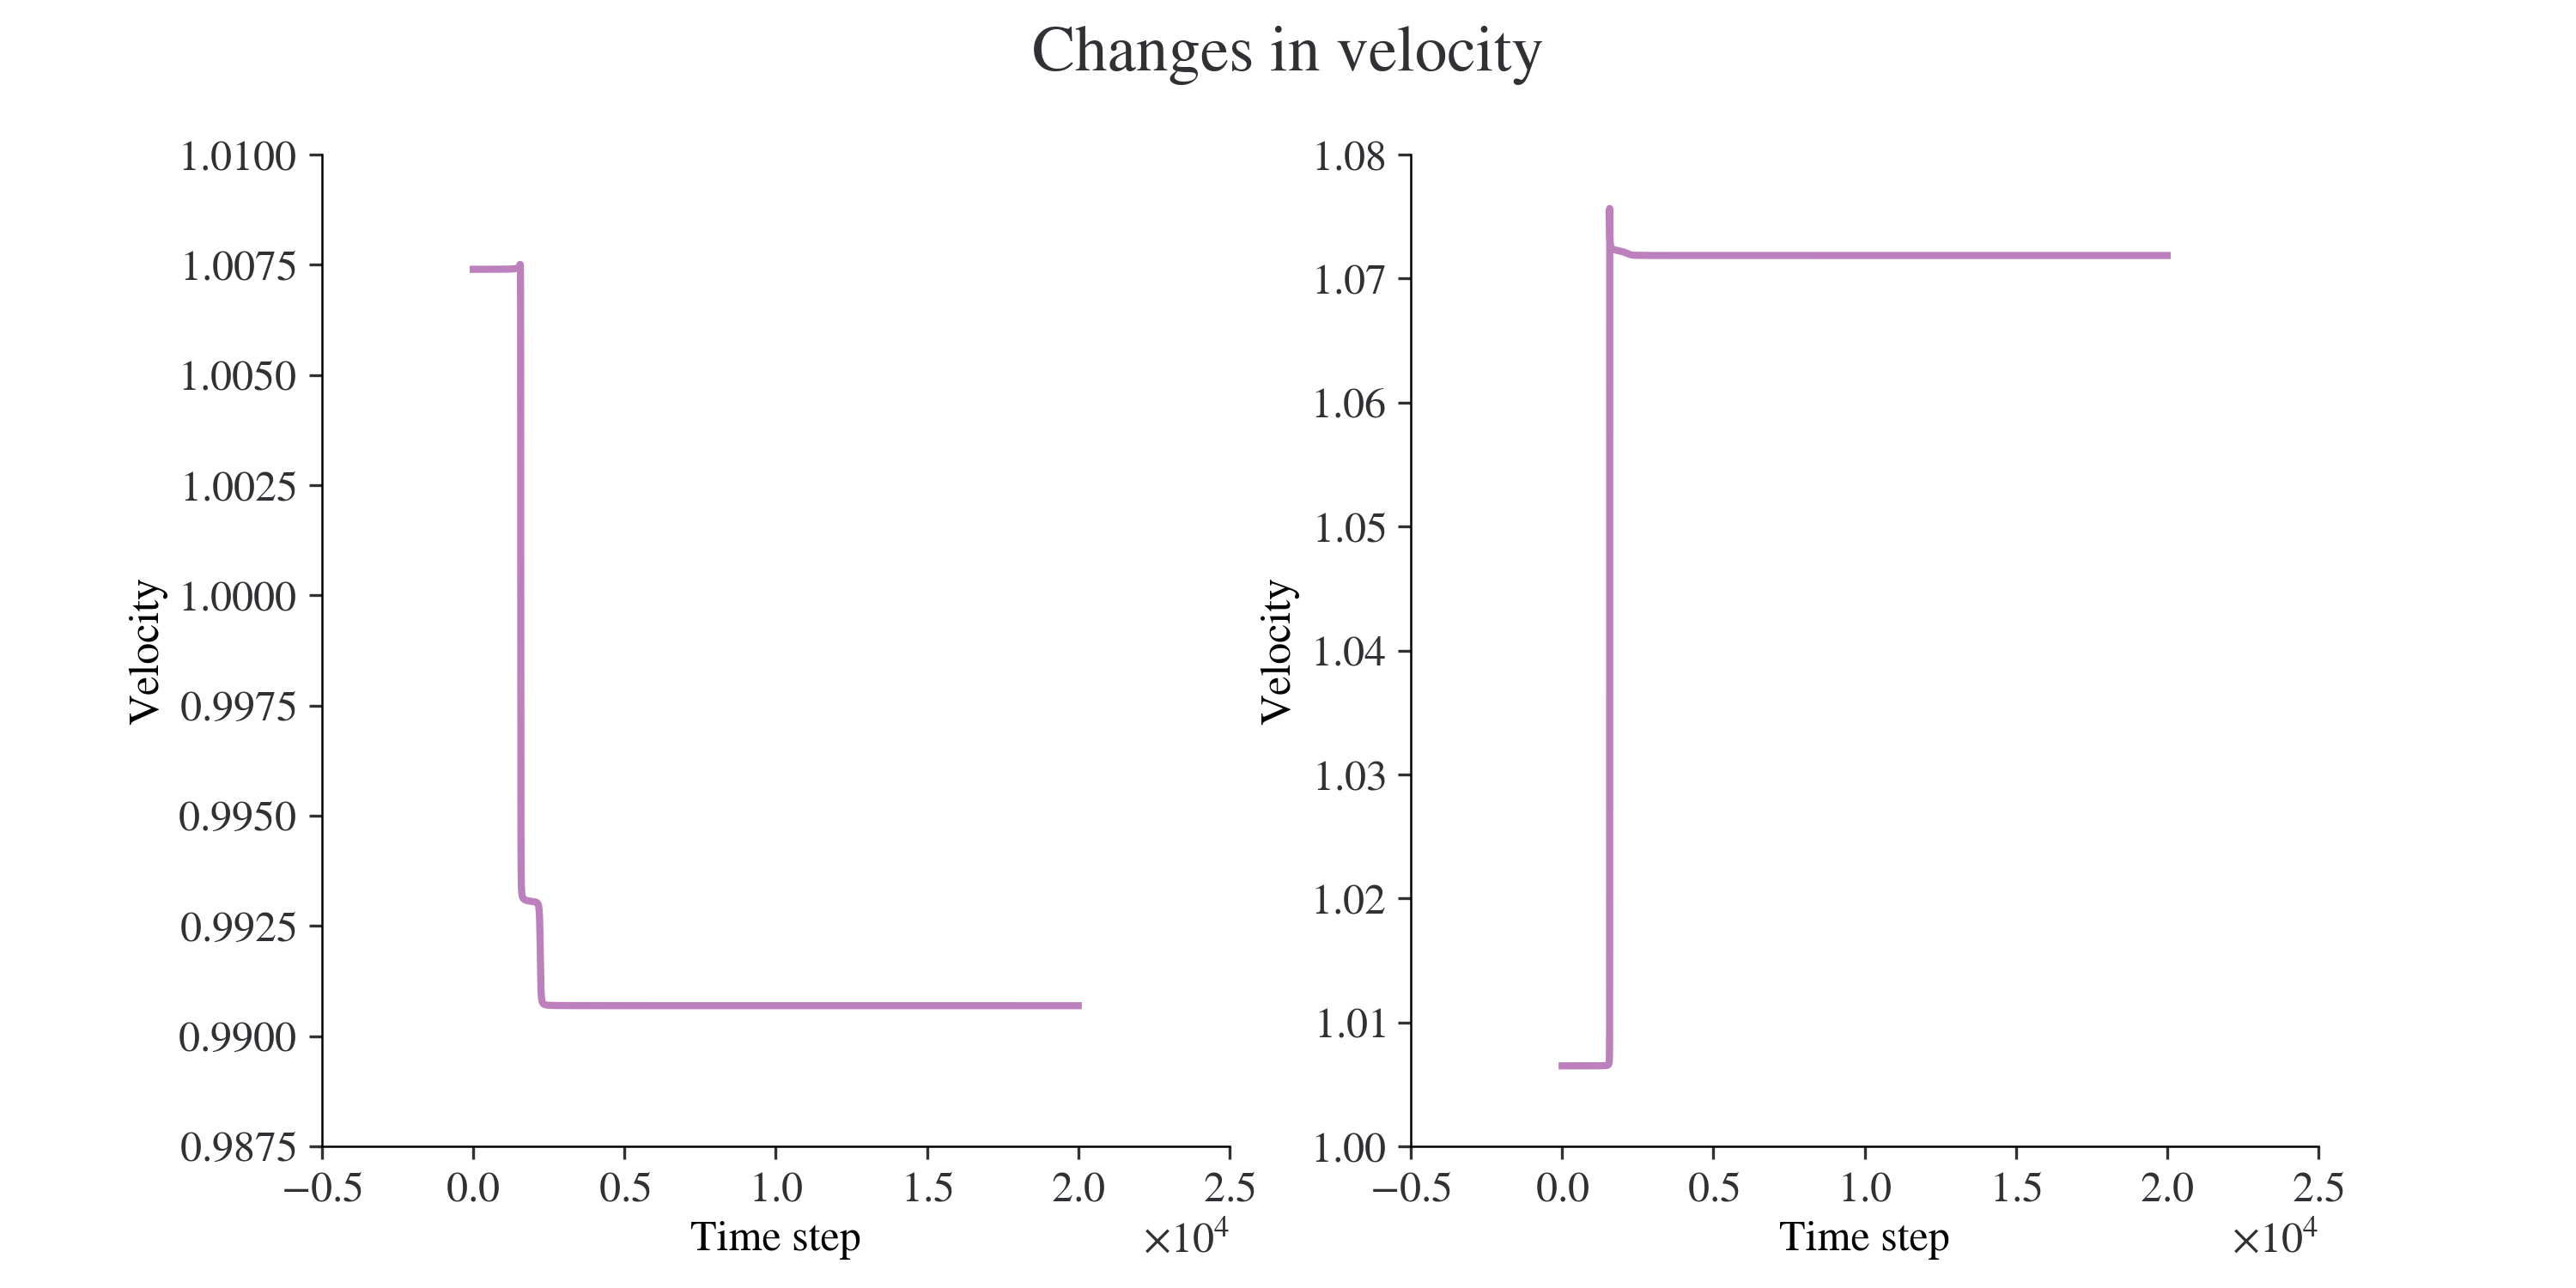
\includegraphics[width=0.7\textwidth]{graphics/earth_velocity_change1.png}
    \caption{Velocity changes during the first gravity assist implementation}
    \label{fig:earth_change1}
\end{figure}


\normalsize{\noindent For the first part of the further investigation, the method outlined yielded some good results, which is demonstrated in Figure \ref{fig:earth_increase1.png}, and a similar simulation was observed for the reduction of velocity case. Figure \ref{fig:earth_change1} also shows a small but noticeable change in velocities in both cases. Energy was also conserved, with an identical graph to \ref{fig:3b_conservation} produced in each case going forward.

\begin{figure}[ht]
    \centering
    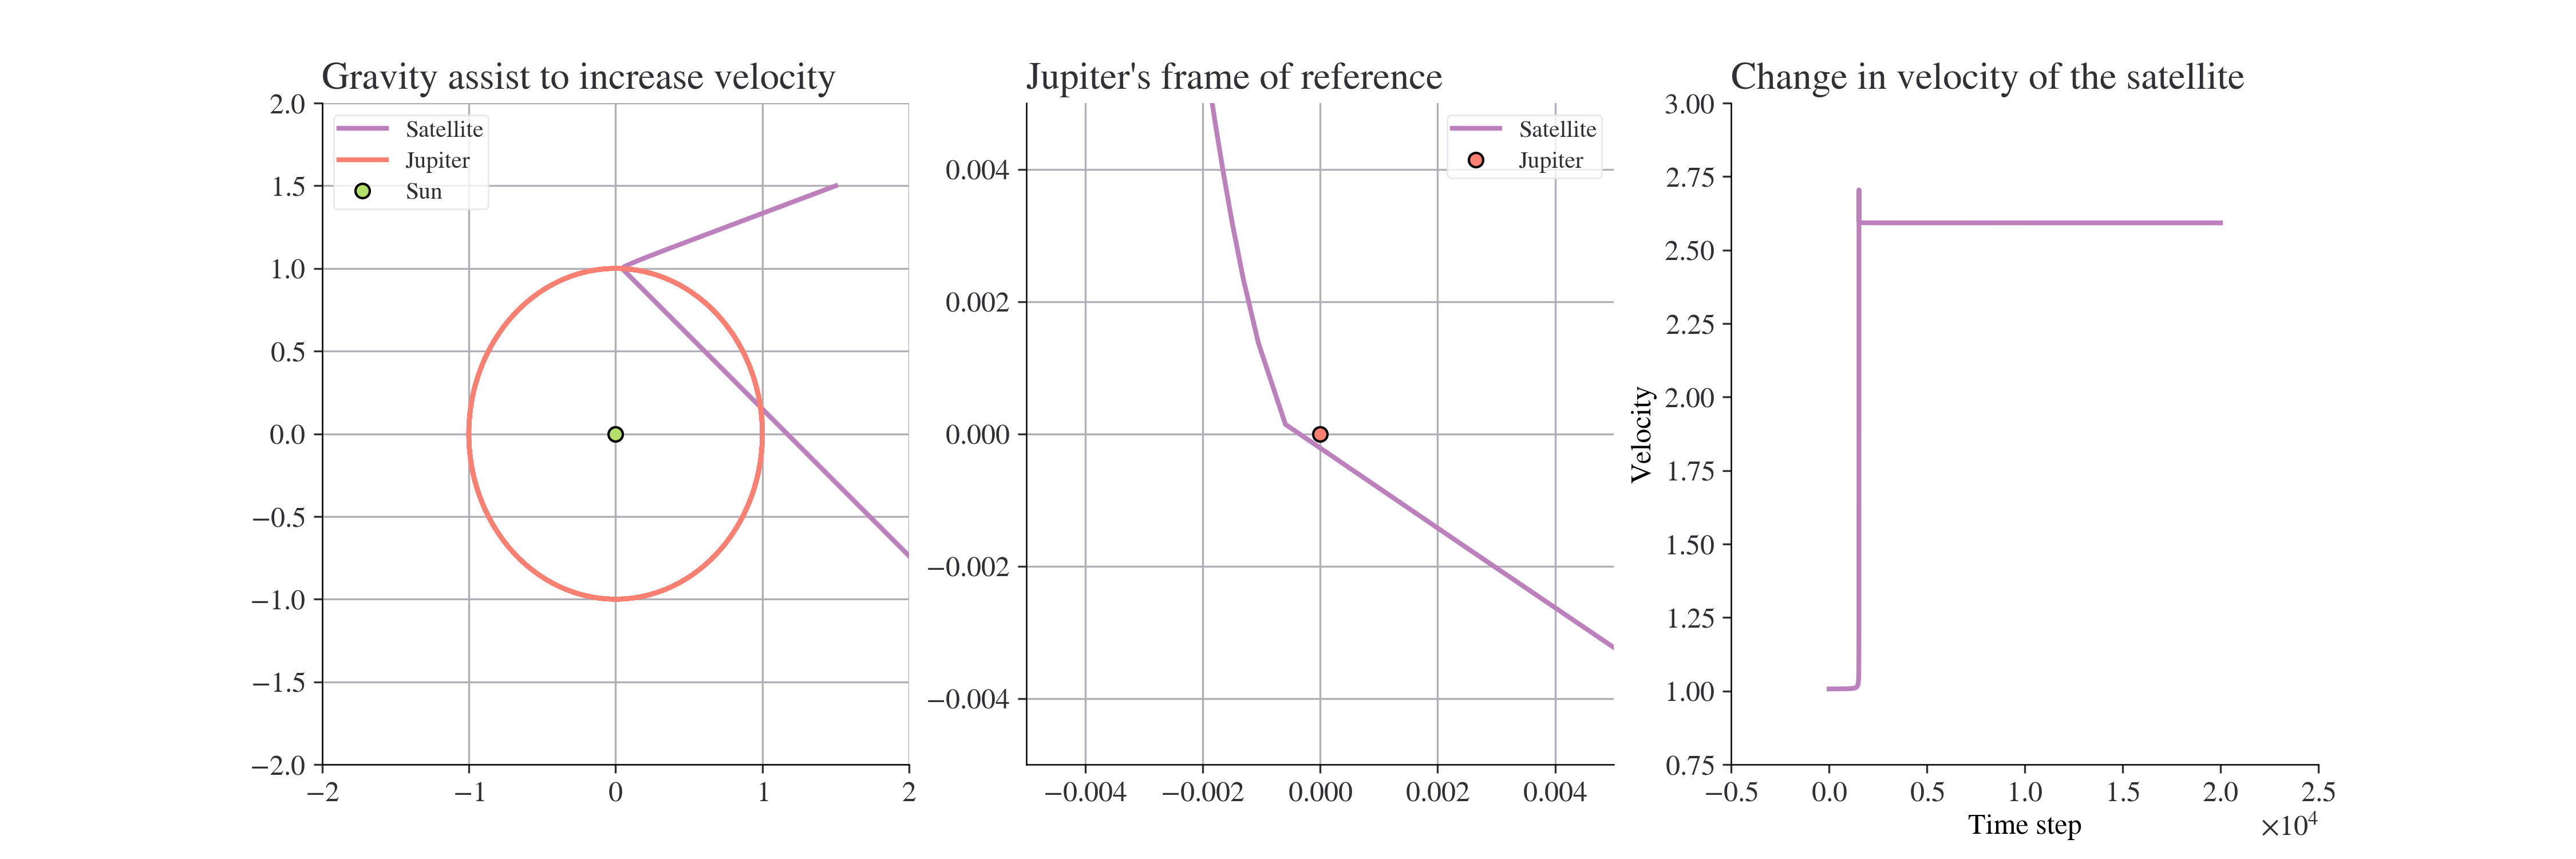
\includegraphics[width=0.9\textwidth]{graphics/jupiter_big_increase.png}
    \caption{A large velocity increase after switching Earth to Jupiter}
    \label{fig:jupiter_big_increase}
\end{figure}

The next part of the investigation concluded that more extreme effects could be realised by considering a larger mass (Jupiter). At this stage, one of the largest hurdles of the simulation became apparent: the time step. Attempts to reduce the time step increased the computational time as expected, but too low of a time step resulted in the planet moving too far between each step to accurately model a gravity assist. Figure \ref{fig:jupiter_big_increase} showcases this. Though a 2.5 times increase is observed, the path in Jupiter's frame of reference is not smooth, which is believed to be due to the time step being too large. An approach that could be taken in future investigations could involve varying time step by multiplying it by the distance ($<1$) between the two planets if it goes below a certain threshold. This would ensure that the key parts of the simulation (when the planets are closer together) are modelled with greater accuracy. Like the case in Figure \ref{fig:jupiter_big_increase}, the alternative trajectory that passed in front of Jupiter also resulted in a substantial decrease in velocity, as one would expect.

\begin{figure}[ht]
    \centering
    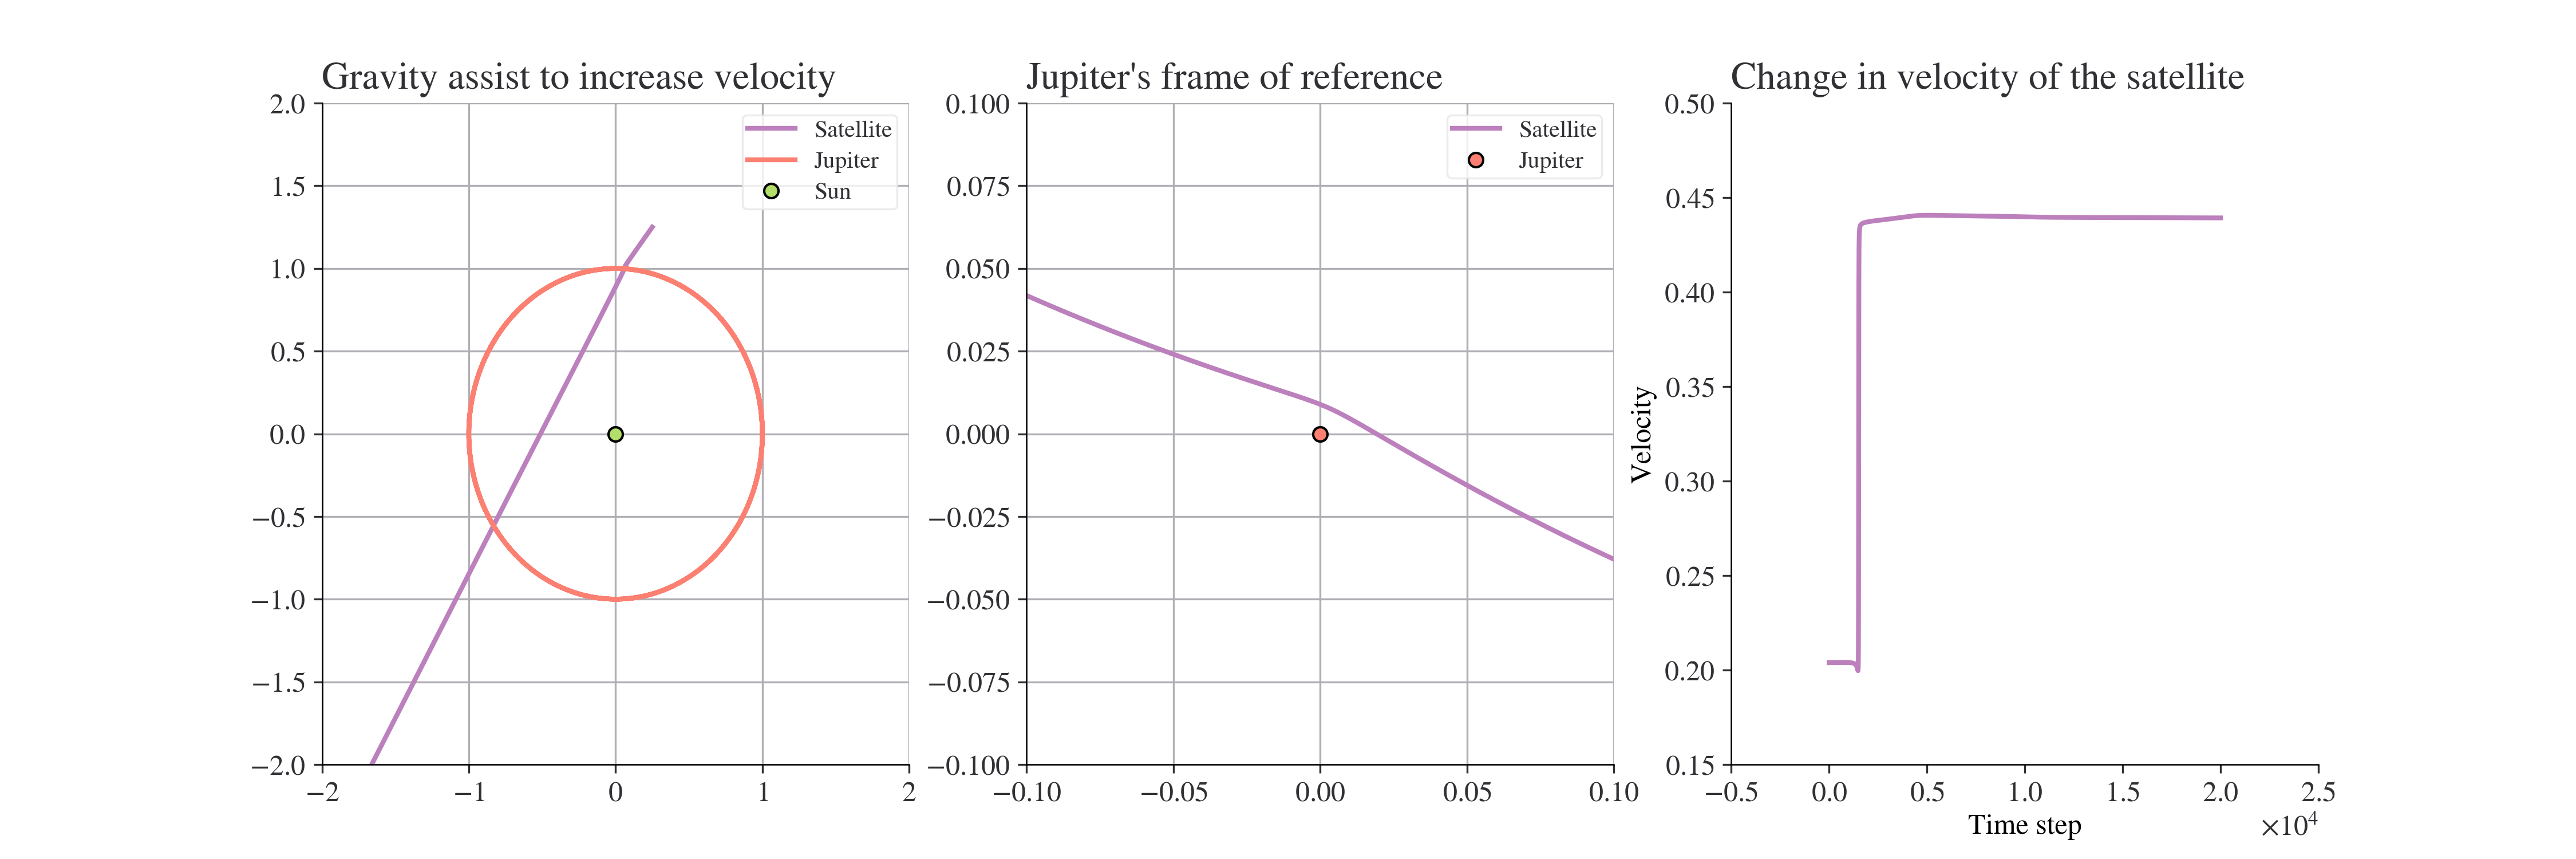
\includegraphics[width=0.9\textwidth]{graphics/jupiter_reduced_vel.png}
    \caption{Another large velocity increase, but this time with a more stable simulation}
    \label{fig:jupiter_reduced_vel}
\end{figure}

In order to attempt to reduce these effects, the satellite was placed at a closer distance to the interception point. For it to reach the interception point at the same time, this required a lower velocity, which was hoped to produce a significant slingshot without having to travel go as far into Jupiter's sphere of influence. It is shown in Figure \ref{fig:jupiter_reduced_vel} that this is possible, with a similar increase to Figure \ref{fig:jupiter_big_increase} but with a smoother and more stable simulation. This was also the case when passing the satellite in front of Jupiter, where it experienced a smooth yet powerful gravity assist.

\begin{figure}[ht]
    \centering
    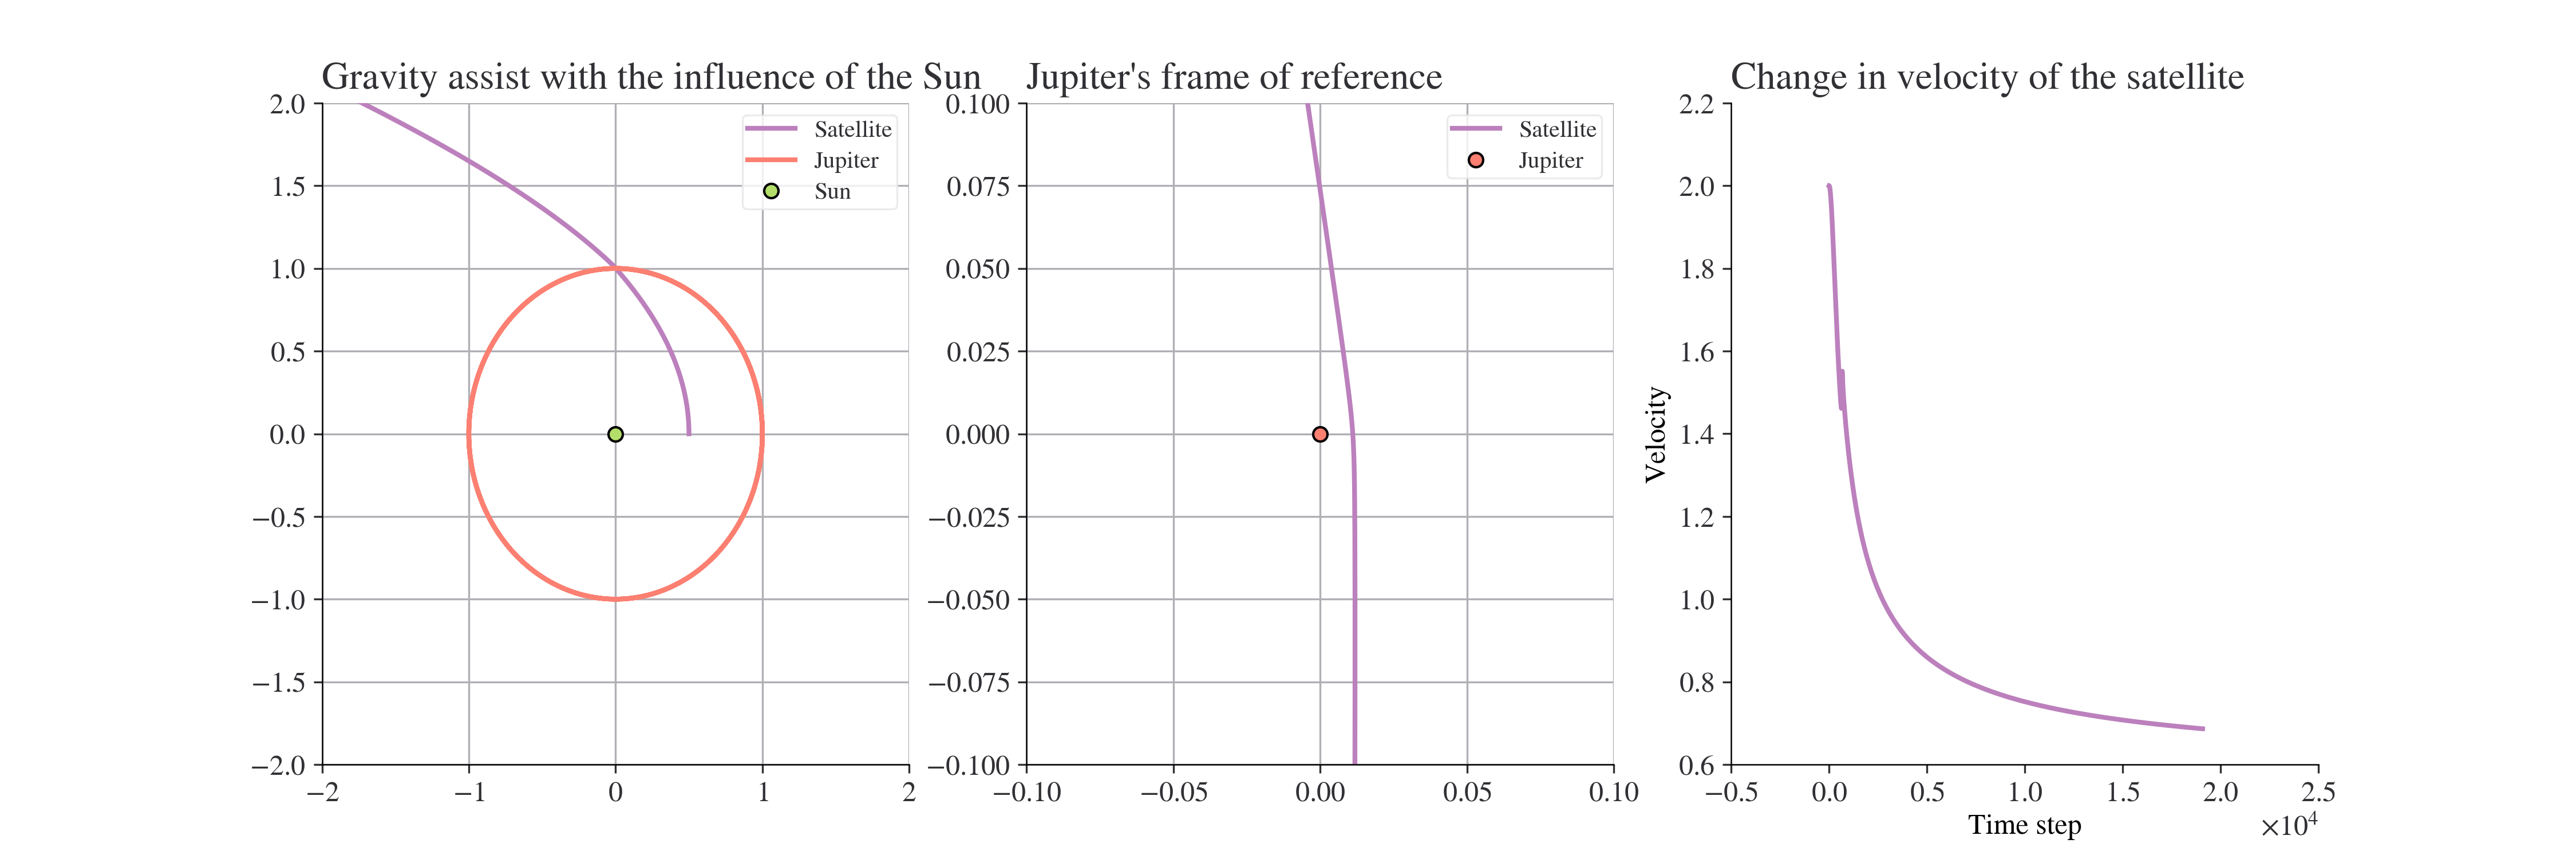
\includegraphics[width=0.9\textwidth]{graphics/circularmotion.png}
    \caption{Gravity assist without neglecting the force on the satellite from the Sun}
    \label{fig:circularmotion}
\end{figure}

When it came to reconsidering the Sun's influence on the satellite, there were some issues in determining how to move it from its initial position to the interception point. Assigning initial velocity no longer sufficed, so doing so with a parabolic orbit (as was mentioned in the previous chapter) was considered a viable option. With a future simulation that is able to harness more computing power, a function could be implemented to determine the parameters for a parabolic or elliptical orbit that intercepts the planet given its initial position. It sufficed with this simulation to determine a working orbit (in this case parabolic), and delaying the satellite's deployment such that it intercepts Jupiter at the assigned interception point. Figure \ref{fig:circularmotion} shows this, though the fact that the system is now perturbed by lag makes it slightly harder to adjust to facilitate increases in velocity. This would be another issue that would be fixed by having a varying time step. Furthermore, in Figure \ref{fig:circularmotion}, it is noticeable that although there is a spike where the gravity assist occurs, the velocity decreases over time. This is due to the gravitational "tailwind" that the satellite experiences as a result of its motion away from the Sun.

\begin{figure}[ht]
    \centering
    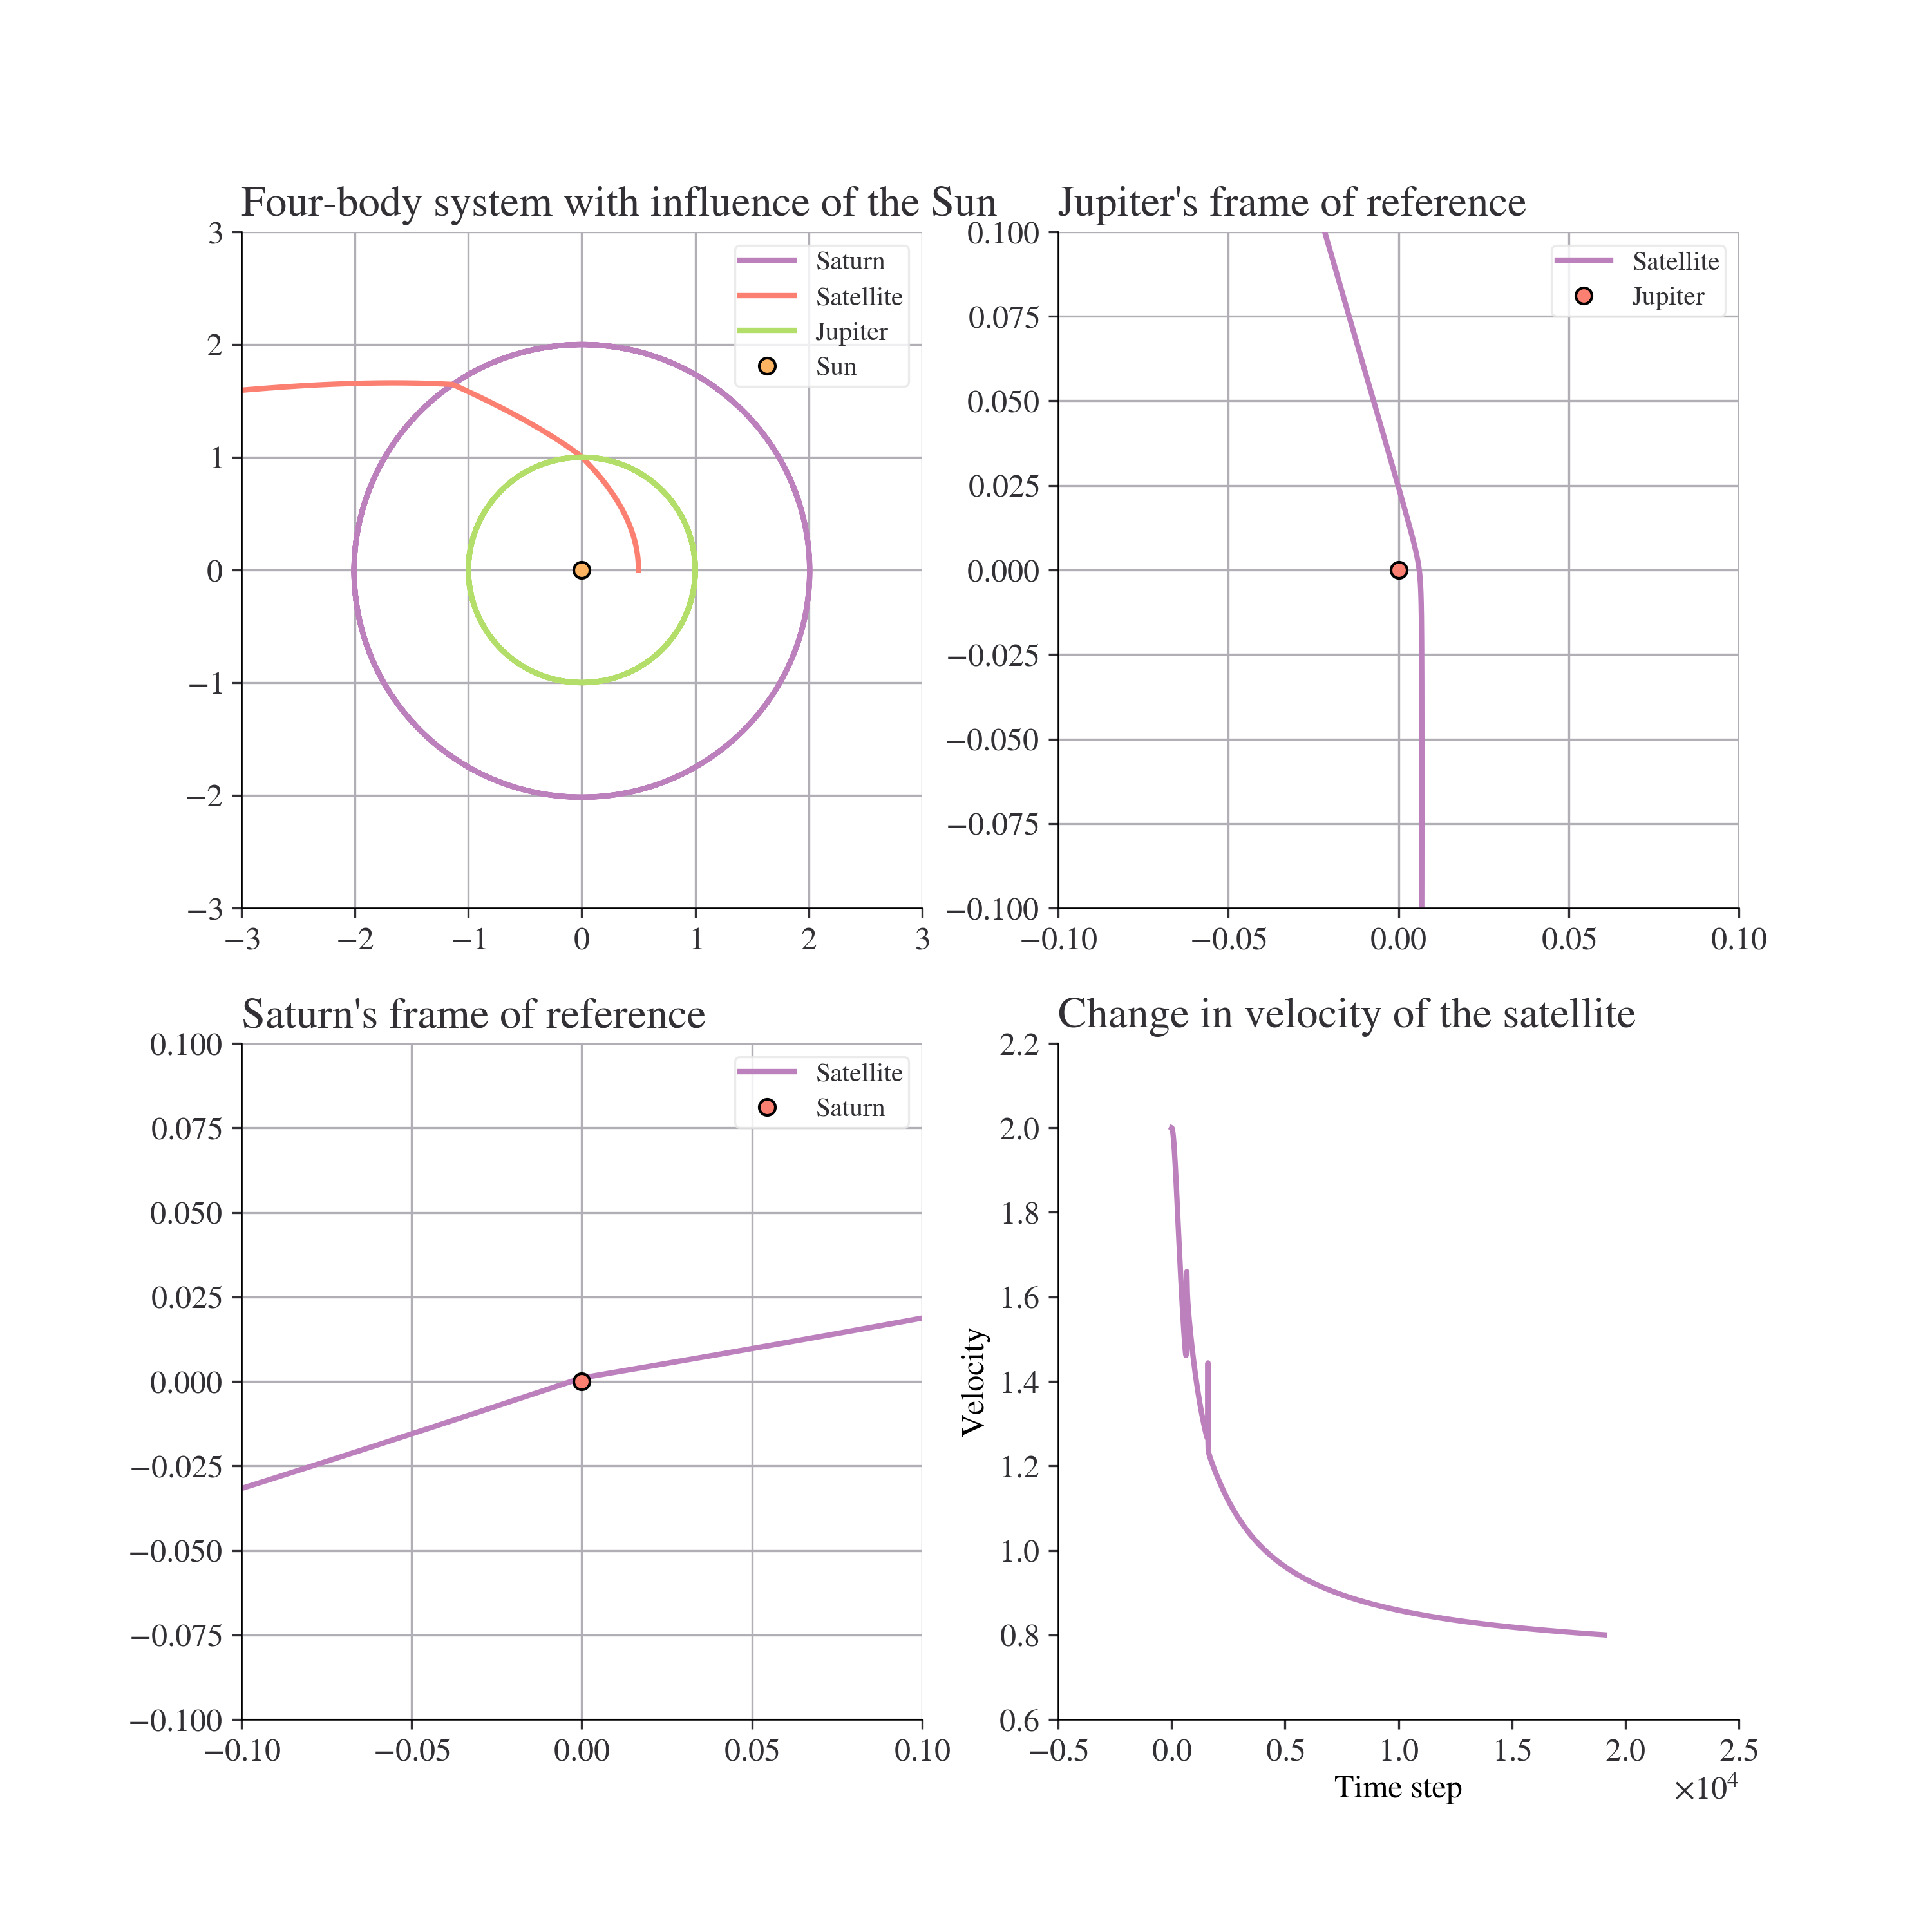
\includegraphics[width=0.9\textwidth]{graphics/fourbody.png}
    \caption{Gravity assist without neglecting the force on the satellite from the Sun}
    \label{fig:fourbody}
\end{figure}

When it came to the final part of the further investigation, a fourth body (Saturn) was introduced. The method used for it to reach the satellite was the same as the method used for the satellite to reach the interception point, and the perturbation of the delay allowed for different trajectories and therefore velocities post-slingshot. As can be seen in Figure \ref{fig:fourbody}, there is a second spike in the velocity where Saturn performs a gravity assist on the satellite. The shape of the graph is very similar to that in Figure \ref{fig:circularmotion}, which one would expect due to the Sun's gravitational pull on the satellite. Both assists contributed to a substantial increase in the velocity of the satellite each time, and it is evident from this that many more bodies could be added without a reduction in the quality of the simulation.
}

\section{\textsl{Other opportunities for exploration}}
\normalsize{\noindent While the simulation from the first assist off Earth up to the two assists off Jupiter and Saturn were adequate, there are a few opportunities to improve upon the realism of these simulations. The first and most obvious point would be the introduction of elliptical orbits to replace the presently circular orbits in the simulation. While this would require usage of different formulae, it is by no means too much of a change from the current simulation, so it appears feasible. Given the problems that were previously mentioned relating to time step, it is difficult to achieve precise trajectories that do not require the perturbation of the system to carry out. The solution and possible implementation of it was discussed in the previous section by using a varying time step. Another interesting method in which the simulation can be developed is through the introduction of interstellar transport. While sounding complex, a simple model alike to this one can be made with the change of reference frame to the Milky Way, and the introduction of one or maybe more solar systems. This would obviously require more computational power but could be executed well with the varying time step idea, or alternatively by using parallel processing. Finally, one more idea that came to mind is the idea of a powered flyby or an Oberth maneuver, as all this requires is the implementation of thrust to the small object. }

%\input{}

\chapter{\textsl{Conclusions}}

\normalsize{\noindent This project aimed to simulate gravity assists under different scenarios in order to understand how a complex astrodynamical maneuver can be simulated in a high level programming language. It succeeded in modelling scenarios ranging from a satellite merely being deflected by Earth's orbit to a multi-stage gravity assist from Jupiter and Saturn. Computational power became a clear issue early into the investigation, but numerous feasible suggestions were made (varying time step or parallel processing) to mitigate this. Nonetheless, with the success of this project, it was suggested also that more complex maneuvers involving thrust are attempted, or greater realism is pursued with the usage of elliptical orbits instead of circular orbits. Overall, high-level programming languages are versatile enough to handle complex astrodynamical simulations, and there is much room to explore more challenging scenarios.}

%\input{}

%%TC:ignore

\addtocontents{toc}{\cftpagenumberson{chapter}}
\addcontentsline{toc}{chapter}{\textbf{References}}
\printbibliography
\clearpage

\renewcommand{\thefigure}{\Alph{chapter}.\arabic{figure}}
\renewcommand{\thetable}{\Alph{chapter}.\arabic{table}}

\updatechaptername
%\input{}

\end{document}
